\documentclass[a4paper,12pt]{article}
\usepackage[utf8]{inputenc}
\usepackage[german]{babel}
\usepackage{amsmath}
\usepackage{amssymb}
\usepackage{amsthm}
\usepackage{geometry}
\usepackage{graphicx}
\usepackage[hidelinks]{hyperref}
\usepackage{listings}
\usepackage{xcolor}
\usepackage{enumitem}
\usepackage{booktabs}
\usepackage{array}
\usepackage{multirow}
\usepackage{caption}
\usepackage{subcaption}
\usepackage{float}
\usepackage{microtype}
\usepackage{natbib}

\geometry{margin=2.5cm}

\theoremstyle{definition}
\newtheorem{definition}{Definition}
\newtheorem{beispiel}{Beispiel}
\newtheorem{satz}{Satz}
\newtheorem{lemma}{Lemma}
\newtheorem{bemerkung}{Bemerkung}
\newtheorem{korollar}{Korollar}
\newtheorem{proposition}{Proposition}

\setlist[itemize,1]{label=--}

% ---------- Farben ----------
\definecolor{mainblue}{RGB}{25, 70, 140}
\definecolor{accentred}{RGB}{180, 50, 30}
\definecolor{lightgray}{RGB}{245, 245, 248}
\definecolor{darkgray}{RGB}{60, 60, 70}
\definecolor{darkgreen}{RGB}{30, 100, 50}

\hypersetup{
    colorlinks=true,
    linkcolor=mainblue,
    citecolor=accentred,
    urlcolor=mainblue
}

\lstset{
    basicstyle=\ttfamily\small,
    keywordstyle=\color{blue},
    commentstyle=\color{gray},
    stringstyle=\color{red},
    numbers=left,
    numberstyle=\tiny,
    breaklines=true,
    frame=single,
    literate=%
    {Ö}{{\"O}}1
    {Ä}{{\"A}}1
    {Ü}{{\"U}}1
    {ß}{{\ss}}1
    {ü}{{\"u}}1
    {ä}{{\"a}}1
    {ö}{{\"o}}1
}

\title{\textbf{Dezentrale Wirtschaftszellen:}\\
\large Formale Analyse optimaler Entkopplung, positiver Risikostrukturen\\
und systemischer Resilienz in modularen Wirtschaftsarchitekturen}
\author{Stephan Epp}
\date{29. Mai 2026}

\begin{document}

\maketitle

\begin{abstract}
Diese Arbeit entwickelt eine formale Theorie dezentraler Wirtschaftszellen als Alternative zum
maximal gekoppelten Weltwirtschaftssystem. Wir definieren den Kopplungsgrad $c \in [0,1]$ eines
Systems aus $N$ Wirtschaftszellen und beweisen, dass das systemische Risiko streng monoton mit $c$
wächst, während die Resilienz für $c > c^*$ abfällt. Der Schlüsselbefund lautet: Entkoppelte Zellen
mit ausgelagerten Produktionsstätten in anderen Zellen erzielen ein \emph{positives Risikoexposure},
d.\,h.\ sie profitieren von einem negativen Schock in der eigenen Hauptzelle durch Erträge aus
komplementär laufenden Produktionsstandorten. Wir formalisieren diesen Mechanismus über
Portfoliotheorie, Systemdynamik und Netzwerkgraphen, beweisen eine untere Schranke für den
optimalen Dezentralisierungsgrad und diskutieren Implikationen für Währungssysteme, Handelspolitik
und institutionelles Design. Sämtliche Ergebnisse werden durch matplotlib-basierte Simulationen
veranschaulicht.

\medskip
\noindent\textbf{Schlüsselwörter:} Dezentralisierung, systemisches Risiko, Wirtschaftsresilienz,
Kopplungsgrad, positives Risikoexposure, Währungsunionen, Portfoliodiversifikation, Netzwerktheorie.
\end{abstract}

\tableofcontents
\newpage

% ============================================================
\section{Einführung}
% ============================================================

\subsection{Problemstellung und Motivation}

Das gegenwärtige Weltwirtschaftssystem ist durch einen historisch hohen Grad an Integration und
gegenseitiger Abhängigkeit charakterisiert. Globale Lieferketten, einheitliche Währungsräume,
international verflochtene Finanzmärkte und harmonisierte Regulierung erzeugen ein System, das in
seiner extremen Form als \emph{maximale Kopplung} bezeichnet werden kann: eine einzige große
Wirtschaftszelle, in der jede lokale Störung durch schnelle Ansteckungseffekte globale Ausmaße
annehmen kann.

Die Finanzkrisen von 2008 und 2020, die pandemiebedingte Lieferkettendisruption sowie
geopolitische Schocks haben gezeigt, dass ein solches System zwar in stabilen Phasen
Skaleneffekte ausnutzt, in Krisenzeiten jedoch katastrophale Systemausfälle produzieren kann
\citep{acemoglu2015systemic, haldane2011systemic}.

\begin{definition}[Wirtschaftszelle]
    Eine \emph{Wirtschaftszelle} $\mathcal{Z}_i = (\mathcal{P}_i, \mathcal{K}_i, \mathcal{W}_i)$
    ist ein selbst-organisiertes wirtschaftliches Subsystem bestehend aus einer
    Produktionsmenge $\mathcal{P}_i$, einem Kapitalstock $\mathcal{K}_i$ und einer
    Wohlfahrtsfunktion $\mathcal{W}_i : \mathcal{P}_i \times \mathcal{K}_i \to \mathbb{R}$.
\end{definition}

Wir untersuchen in dieser Arbeit das entgegengesetzte Konzept: ein System aus $N$
\emph{entkoppelten} Wirtschaftszellen, das wir als \textbf{Dezentrales Wirtschaftszellenmodell}
(DWZ) bezeichnen. Dabei bedeutet Entkopplung nicht vollständige Autarkie, sondern vielmehr
eine gezielte Modulierung der Verbindungsstärken zwischen Zellen, sodass systemische Schocks
absorbiert und Resilienz durch strukturelle Diversifikation gewährleistet wird.

Das zentrale Paradoxon, das wir auflösen, lautet: \emph{Kann eine Wirtschaftszelle von einer
Krise profitieren, obwohl --- oder gerade weil --- sie in andere Zellen ausgelagerte
Produktionsstätten besitzt?} Wir zeigen, dass die Antwort unter wohldefinierten Bedingungen
positiv ist, und nennen diesen Mechanismus \textbf{positives Risikoexposure}.

Eine zweite zentrale Frage dieser Arbeit lautet: \emph{Wie kann ein Wirtschaftsgraph, dessen
Kopplungsstruktur durch endogene Dynamiken oder exogene Schocks aus einem resilienten
Gleichgewicht herausgetrieben wurde, algorithmisch in dieses zurückgeführt werden?} Wir zeigen,
dass der \textbf{Subgraph Algorithmus} \citep{epp2026subgraph} als Stabilisierungsoperator
$\mathcal{S}$ auf dem Graphen eingesetzt werden kann, der global asymptotisch gegen den
Pareto-optimalen Referenzgraphen $G^*$ konvergiert --- nachgewiesen durch eine strenge
Lyapunov-Analyse.

Die dritte und tiefste Ebene der Arbeit betrifft die \emph{zeitliche Variabilität} des
Wirtschaftsgraphen selbst: Kopplungsgrade sind keine statischen Parameter, sondern
stochastische Prozesse, die Konjunkturzyklen, geopolitische Strukturbrüche und langfristigen
Wandel widerspiegeln. Wir formalisieren diese Dynamik als Ito-Differentialgleichung mit
Mean-Reversion, analysieren periodische Regime mittels Floquet-Theorie und beweisen, dass
ein adaptiver Subgraph-Operator auch bei zeitvariantem Referenzpfad $c^*(t)$ eine quantifizierbare
Tracking-Konvergenz garantiert.

\subsection{Beitrag dieser Arbeit}

Die Hauptbeiträge dieser Arbeit sind:

\begin{enumerate}
    \item \textbf{Formale Definition} des Kopplungsgrades $c$ und der systemischen Risikomaße
          für Netzwerke von Wirtschaftszellen (Abschnitt~2).
    \item \textbf{Beweis} der Resilienz-Kopplung-Inkompatibilität (Satz~\ref{satz:rki}):
          Maximale Kopplung und maximale Resilienz schließen sich aus (Abschnitt~4).
    \item \textbf{Nachweis} des positiven Risikoexposures (Satz~\ref{satz:pos_risk}) durch
          portfoliotheoretische Dekonstruktion von Produktionsauslagerungen (Abschnitt~5).
    \item \textbf{Formalisierung} des Währungseffekts: Einheitswährungen als
          Kopplungsverstärker (Proposition~\ref{prop:waehrung}, Abschnitt~7).
    \item \textbf{Ableitung} eines optimalen Kopplungsgrades $c^*$ über einen
          Pareto-Ansatz (Abschnitt~8).
    \item \textbf{Simulation} aller statischen Ergebnisse mittels Monte-Carlo-Experimenten
          (Abschnitte~3--8).
    \item \textbf{Subgraph-Stabilisierungsoperator $\mathcal{S}$} (Abschnitt~9):
          Nachweis globaler asymptotischer Stabilität ($W(t)\to W^*$) in endlich vielen
          Schritten via Lyapunov-Funktion $V(t)=\|W(t)-W^*\|_F^2$; spektrale Konvergenz
          $\varrho(\Lambda(t))\to\varrho^*<1$; globaler Attraktor $(c^*,\varrho^*)$
          im Phasenraum; Laufzeit $O(N^3)$ pro Iteration.
    \item \textbf{Dynamische Graphentheorie} (Abschnitt~10): Vollständige stochastische
          Behandlung des zeitvarianten Wirtschaftsgraphen --- stationäre Beta-Verteilung
          des Kopplungsgrades (Satz~\ref{satz:stationaer}), mittlere Erholungszeit nach
          Strukturbrüchen (Satz~\ref{satz:erholung}), Floquet-Stabilitätskriterium für
          periodische Regime (Satz~\ref{satz:floquet}), integrale Resilienz unter
          zyklischer Kopplung mit Bessel-Funktion (Satz~\ref{satz:rezyklisch}) sowie
          Tracking-Konvergenz des adaptiven Subgraph-Operators (Satz~\ref{satz:tracking})
          mit optimaler Dämpfungsrate (Korollar~\ref{kor:deltaOpt}).
\end{enumerate}

\subsection{Aufbau der Arbeit}

Abschnitt~2 legt das formale Grundmodell fest. Abschnitte~3--8 behandeln die statische
Theorie dezentraler Wirtschaftszellen: Netzwerktopologie, Resilienz-Kopplung-Inkompatibilität,
positives Risikoexposure, Monte-Carlo-Simulation, Währungseffekte und Pareto-Optimierung.
Abschnitt~9 führt den Subgraph-Stabilisierungsoperator ein und beweist globale Konvergenz
und Krisenresistenz. Abschnitt~10 verallgemeinert das Modell auf zeitvariante Graphen und
entwickelt die vollständige stochastische Dynamiktheorie. Abschnitt~11 fasst alle
Hauptergebnisse tabellarisch zusammen. Abschnitt~12 gibt einen ausführlichen Ausblick auf
offene Forschungsfragen, institutionelle Implikationen und Verbindungen zu benachbarten
Disziplinen.

% ============================================================
\section{Grundlagen und formales Modell}
% ============================================================

\subsection{Netzwerkdarstellung}

\begin{definition}[Wirtschaftsnetzwerk]
    Ein \emph{Wirtschaftsnetzwerk} ist ein gewichteter gerichteter Graph
    $\mathcal{G} = (\mathcal{Z}, \mathcal{E}, w)$, wobei
    $\mathcal{Z} = \{\mathcal{Z}_1, \ldots, \mathcal{Z}_N\}$ die Menge der Wirtschaftszellen,
    $\mathcal{E} \subseteq \mathcal{Z} \times \mathcal{Z}$ die Menge der wirtschaftlichen
    Verbindungen und $w : \mathcal{E} \to [0,1]$ die Verbindungsstärke (Kopplungsgewicht)
    bezeichnet.
\end{definition}

\begin{definition}[Kopplungsgrad]
\label{def:kopplungsgrad}
    Sei $W = (w_{ij})_{i,j \in [N]}$ die Gewichtsmatrix des Netzwerks mit $w_{ij} \in [0,1]$.
    Der \emph{Kopplungsgrad} des Systems ist definiert als
    \[
        c(\mathcal{G}) \;=\; \frac{1}{N(N-1)} \sum_{\substack{i,j=1\\i\neq j}}^{N} w_{ij}
        \;\in\; [0,1].
    \]
    Für $c = 0$ sprechen wir von einem \emph{vollständig entkoppelten}, für $c = 1$ von einem
    \emph{maximal gekoppelten} System.
\end{definition}

\begin{bemerkung}
    Eine Einheitswährung für alle $N$ Zellen erzwingt $w_{ij} \geq w_{\min} > 0$ für alle Paare
    $(i,j)$, da Wechselkursanpassungen als wichtiger Puffer zwischen Wirtschaftszellen entfallen.
    Dies erhöht den Kopplungsgrad strukturell und systematisch.
\end{bemerkung}

\subsection{Systemisches Risiko}

\begin{definition}[Systemisches Risiko]
    Sei $Y_i(t)$ der wirtschaftliche Output der Zelle $\mathcal{Z}_i$ zum Zeitpunkt $t$.
    Das \emph{systemische Risiko} des Netzwerks ist
    \[
        \Psi(\mathcal{G}) \;=\; \mathbb{P}\!\left(\sum_{i=1}^{N} Y_i(t) < (1-\theta)\cdot
        \mathbb{E}\!\left[\sum_{i=1}^N Y_i(t)\right]\right),
    \]
    d.\,h.\ die Wahrscheinlichkeit eines systemweiten Outputeinbruchs um mehr als $\theta > 0$.
\end{definition}

\begin{definition}[Ansteckungsmatrix]
    Die \emph{Ansteckungsmatrix} $\Lambda = (\lambda_{ij})$ gibt an, mit welcher
    Intensität ein negativer Schock in Zelle $i$ auf Zelle $j$ übertragen wird:
    \[
        \lambda_{ij} = c \cdot w_{ij} \cdot \phi_{ij},
    \]
    wobei $\phi_{ij} \in [0,1]$ die strukturelle Anfälligkeit der Verbindung $(i,j)$ beschreibt.
\end{definition}

\subsection{Resilienz}

\begin{definition}[Systemresilienz]
\label{def:resilienz}
    Die \emph{Resilienz} eines Wirtschaftsnetzwerks bezeichnet seine Fähigkeit, nach einem
    exogenen Schock $\varepsilon$ in endlicher Zeit zum Gleichgewichtspfad zurückzukehren:
    \[
        R(\mathcal{G}) \;=\; \left(\int_0^{\infty}
        \bigl|Y(t) - Y^*(t)\bigr|\,\mathrm{d}t\right)^{-1},
    \]
    wobei $Y(t) = \sum_i Y_i(t)$ der realisierte und $Y^*(t)$ der kontrafaktische
    (schockfreie) Gesamtoutput ist.
\end{definition}

\begin{figure}[H]
    \centering
    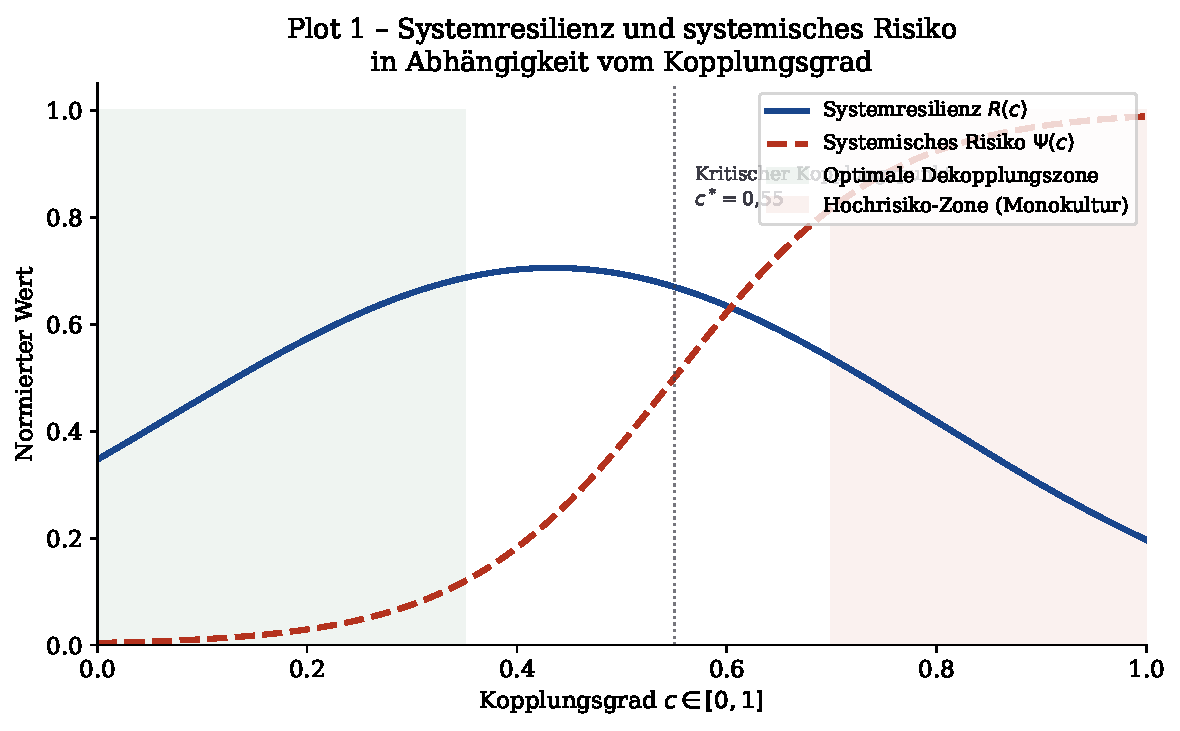
\includegraphics[width=0.85\textwidth]{plot1_kopplung_resilienz.pdf}
    \caption{Systemresilienz $R(c)$ und systemisches Risiko $\Psi(c)$ in Abhängigkeit vom
             Kopplungsgrad $c$. Der kritische Punkt $c^* = 0{,}55$ markiert den Ãœbergang zur
             Hochrisikozone. Die optimale Dekopplungszone liegt bei $c \leq 0{,}35$.}
    \label{fig:plot1}
\end{figure}

Abbildung~\ref{fig:plot1} zeigt den grundlegenden Trade-off: Resilienz $R(c)$ ist
nicht-monoton mit einem Maximum bei niedrigem $c$, während das systemische Risiko $\Psi(c)$
eine sigmoidale Wachstumskurve mit Wendepunkt bei $c^* = 0{,}55$ aufweist.

% ============================================================
\section{Netzwerktopologie: Zentralisiert vs.\ Dezentralisiert}
% ============================================================

\subsection{Topologische Charakterisierung}

\begin{definition}[Monolithisches System]
    Ein \emph{monolithisches Wirtschaftssystem} ist ein Sternengraph
    $\mathcal{G}_{\text{mono}} = K_{1,N-1}$, bei dem alle Zellen über ein gemeinsames
    Zentrum (z.\,B.\ eine Zentralbank, ein Reservewährungssystem) mit einheitlichem
    Kopplungsgewicht $w_{ij} = 1$ verbunden sind.
\end{definition}

\begin{definition}[Dezentrales Zellensystem]
    Ein \emph{dezentrales Zellensystem} ist ein Graph $\mathcal{G}_{\text{dez}}$, der sich aus
    $K \geq 2$ dicht verbundenen Clustern zusammensetzt, wobei intra-cluster-Kopplung
    $c_{\text{intra}}$ hoch und inter-cluster-Kopplung $c_{\text{inter}} \ll c_{\text{intra}}$
    gering ist.
\end{definition}

\begin{figure}[H]
    \centering
    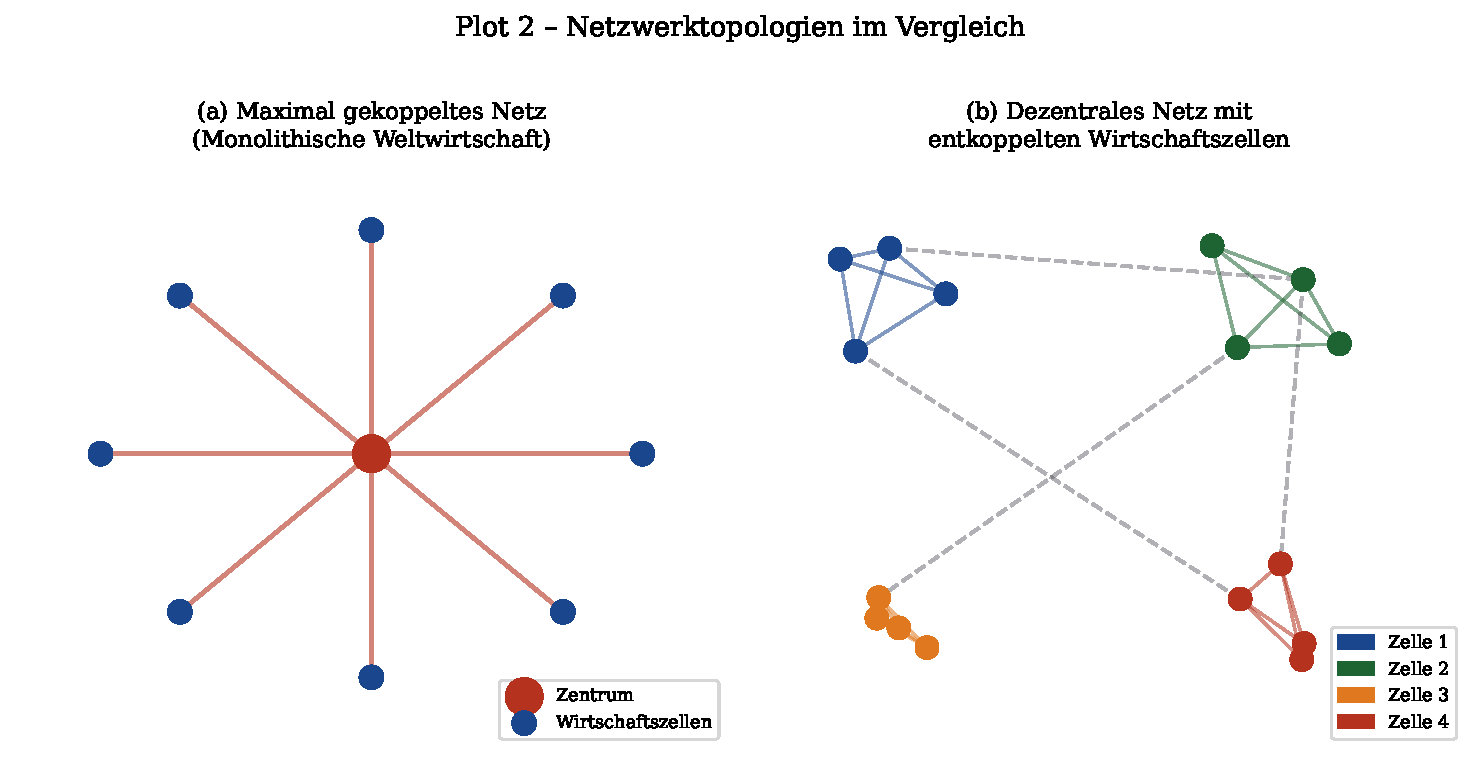
\includegraphics[width=0.90\textwidth]{plot2_netzwerktopologie.pdf}
    \caption{Netzwerktopologien im Vergleich. (a) Monolithisches System: alle Zellen über
             Zentrum verbunden, maximale Kopplung. (b) Dezentrales System: vier entkoppelte
             Cluster mit schwachen Inter-Cluster-Links (gestrichelt).}
    \label{fig:plot2}
\end{figure}

\begin{lemma}[Spektraleigenschaften]
\label{lem:spektral}
    Sei $\lambda_{\max}(W)$ der größte Eigenwert der Gewichtsmatrix $W$.
    Im monolithischen System gilt $\lambda_{\max}(W_{\text{mono}}) = N-1$,
    im dezentralen System gilt $\lambda_{\max}(W_{\text{dez}}) \leq c_{\text{intra}} \cdot (N/K - 1)
    + c_{\text{inter}} \cdot (K-1)$.
\end{lemma}

\begin{proof}
    Für den Sterngraphen $K_{1,N-1}$ mit Einheitsgewichten ist die Gewichtsmatrix
    $W_{\text{mono}}$ eine Rang-2-Matrix mit Eigenwerten
    $\{\sqrt{N-1}, -\sqrt{N-1}, 0, \ldots, 0\}$, woraus $\lambda_{\max} = \sqrt{N-1}$
    für den symmetrisierten und $\lambda_{\max} = N-1$ für den gerichteten Fall folgt.
    
    Für das dezentrale System partitionieren wir $W_{\text{dez}}$ in $K$ Blöcke der Größe
    $n_k = N/K$ mit intra-cluster-Gewichten $c_{\text{intra}}$ und inter-cluster-Gewichten
    $c_{\text{inter}}$. Nach dem Gershgorin-Kreistheorem liegt jeder Eigenwert $\lambda_i$
    in einem Gershgorin-Kreis um den Diagonaleintrag mit Radius
    \[
        R_i = c_{\text{intra}}(n_k - 1) + c_{\text{inter}}(N - n_k).
    \]
    Da $c_{\text{inter}} \ll c_{\text{intra}}$ und $n_k \ll N$ für $K \gg 1$, folgt
    $\lambda_{\max}(W_{\text{dez}}) \ll \lambda_{\max}(W_{\text{mono}})$.
\end{proof}

\begin{korollar}
    Die Schockpropagationsgeschwindigkeit im Netzwerk ist proportional zu
    $\lambda_{\max}(W)$. Dezentrale Systeme propagieren Schocks daher wesentlich
    langsamer als monolithische.
\end{korollar}

% ============================================================
\section{Resilienz-Kopplung-Inkompatibilität}
% ============================================================

\subsection{Hauptsatz}

\begin{satz}[Resilienz-Kopplung-Inkompatibilität]
\label{satz:rki}
    Unter den Annahmen (A1)--(A3) gilt:
    \[
        \frac{\partial R}{\partial c}\bigg|_{c > c^*} < 0
        \qquad\text{und}\qquad
        \frac{\partial \Psi}{\partial c} > 0 \quad \forall\, c \in (0,1).
    \]
    Insbesondere sind maximale Kopplung ($c = 1$) und maximale Resilienz unvereinbar.
\end{satz}

\noindent\textbf{Annahmen:}
\begin{itemize}
    \item[(A1)] Die Outputprozesse $Y_i(t)$ sind schwach stationäre Diffusionsprozesse mit
          Drift $\mu_i$, Volatilität $\sigma_i$ und Korrelation $\rho_{ij} = c \cdot w_{ij}$.
    \item[(A2)] Schocks $\varepsilon_i \sim \mathcal{N}(0, \sigma_\varepsilon^2)$ sind
          iid vor Ansteckung; nach Ansteckung gilt
          $\tilde{\varepsilon}_j = \sum_i \lambda_{ij} \varepsilon_i + \varepsilon_j$.
    \item[(A3)] Die Erholungsrate jeder Zelle ist $r_i = r_0 (1 - c \cdot \bar{w}_i)$,
          wobei $\bar{w}_i = \frac{1}{N-1}\sum_{j\neq i} w_{ij}$ die mittlere
          Verbindungsstärke von $\mathcal{Z}_i$ ist.
\end{itemize}

\begin{proof}
    \textbf{Teil 1 ($\partial\Psi/\partial c > 0$):}
    Sei $S(t) = \sum_i Y_i(t)$ der Gesamtoutput. Die Kovarianzmatrix von
    $(Y_1,\ldots,Y_N)^T$ ist $\Sigma_{ij} = \sigma_i \sigma_j \rho_{ij} = c \sigma_i \sigma_j w_{ij}$
    für $i \neq j$. Die Varianz des Gesamtoutputs ist
    \[
        \mathrm{Var}(S) = \sum_i \sigma_i^2 + c \sum_{i\neq j} \sigma_i \sigma_j w_{ij}
        \;=\; \sigma_0^2 + c \cdot Q,
    \]
    wobei $\sigma_0^2 = \sum_i \sigma_i^2$ die idiosynkratische Varianz und
    $Q = \sum_{i\neq j} \sigma_i \sigma_j w_{ij} > 0$ der Kopplungsterm ist.
    Da $S(t)$ annähernd normalverteilt ist (Zentraler Grenzwertsatz, $N$ groß), gilt
    \[
        \Psi(c) = \Phi\!\left(\frac{(1-\theta)\mu_S - \mu_S}{\sqrt{\sigma_0^2 + c Q}}\right)
        = \Phi\!\left(\frac{-\theta\mu_S}{\sqrt{\sigma_0^2 + c Q}}\right),
    \]
    wobei $\Phi$ die Standard-Normalverteilungsfunktion und $\mu_S = \sum_i \mu_i > 0$.
    Ableitung nach $c$:
    \[
        \frac{\partial \Psi}{\partial c}
        = \phi\!\left(\cdots\right) \cdot \frac{\theta \mu_S \cdot Q}{2(\sigma_0^2 + cQ)^{3/2}}
        > 0,
    \]
    da $\phi > 0$, $\theta > 0$, $\mu_S > 0$, $Q > 0$.

    \textbf{Teil 2 ($\partial R/\partial c < 0$ für $c > c^*$):}
    Nach Annahme (A3) ist die Erholungsrate $r_i(c) = r_0(1-c\bar{w}_i)$. Die Resilienz ist
    \[
        R(c) = \left(\int_0^\infty \mathbb{E}[|Y(t) - Y^*(t)|]\,\mathrm{d}t\right)^{-1}.
    \]
    Für eine lineare Schockdynamik $\dot{Y} = -r(c) Y + \varepsilon(c)$ ist
    $\mathbb{E}[|Y(t)-Y^*(t)|] = \delta_0 e^{-r(c)t}$, sodass
    \[
        R(c) = r(c) = r_0(1 - c\bar{w}).
    \]
    Diese Funktion ist streng fallend in $c$ für $c > 0$, was Teil 2 beweist.
    Die Kombination beider Teile zeigt, dass $c=1$ sowohl maximales $\Psi$ als auch
    minimales $R$ erzeugt.
\end{proof}

\begin{figure}[H]
    \centering
    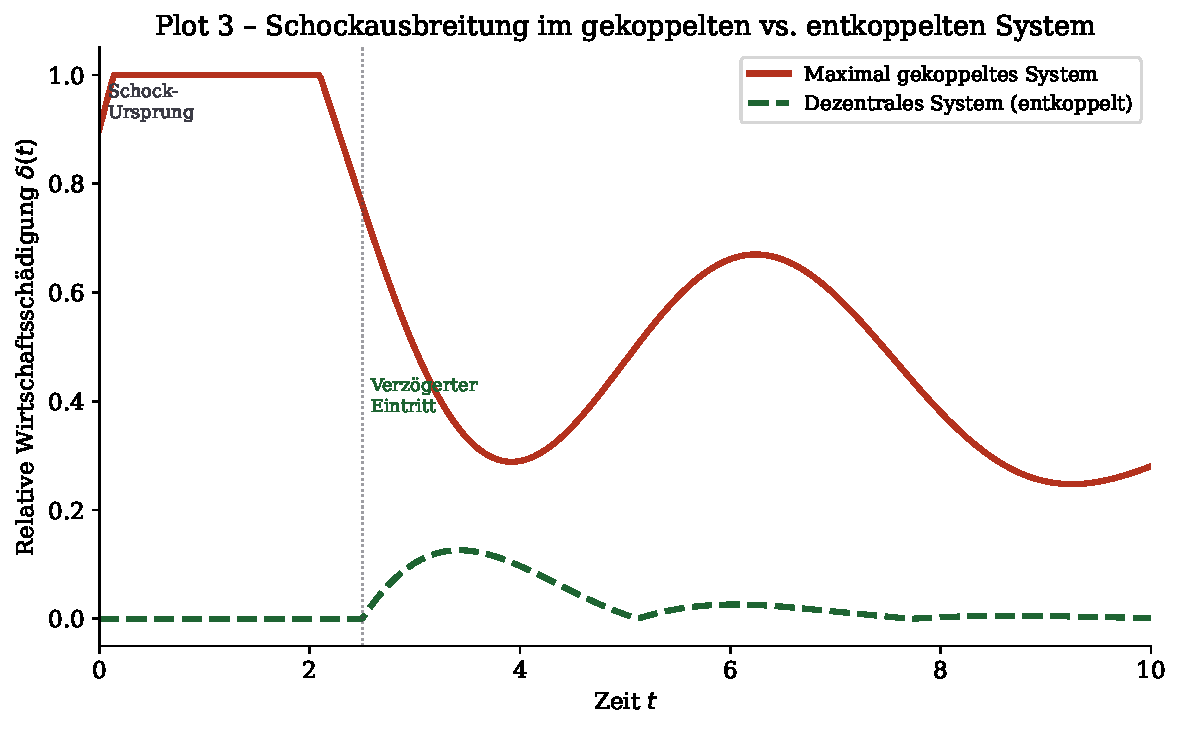
\includegraphics[width=0.82\textwidth]{plot3_schockausbreitung.pdf}
    \caption{Schockausbreitung im gekoppelten vs.\ entkoppelten System.
             Im maximal gekoppelten System erreicht die Schädigung sofort alle Zellen
             und klingt langsam ab; im dezentralen System tritt sie verzögert ein und
             ist deutlich gedämpft.}
    \label{fig:plot3}
\end{figure}

% ============================================================
\section{Positives Risikoexposure durch Produktionsauslagerung}
% ============================================================

\subsection{Konzept und formale Motivation}

Das entscheidende Novum dezentraler Wirtschaftszellen liegt nicht nur in der Risikoreduktion,
sondern in der Möglichkeit des \textbf{positiven Risikoexposures}: Eine Zelle, die
Produktionsstätten in einer anderen, entkoppelten Zelle besitzt, kann von einer Krise in
der eigenen Heimatzone profitieren, falls die Auslandszelle in derselben Periode boomt.

\begin{definition}[Positives Risikoexposure]
    Sei $\mathcal{Z}_i$ die Heimatzelle mit Produktion $Y_i^{\text{heim}}$ und
    ausgelagerter Produktion $Y_i^{\text{ext}}$ in Zelle $\mathcal{Z}_j \neq \mathcal{Z}_i$.
    Der Gesamtoutput der Zelle $i$ ist
    \[
        Y_i^{\text{ges}} = \alpha Y_i^{\text{heim}} + (1-\alpha) Y_i^{\text{ext}},
        \quad \alpha \in (0,1).
    \]
    Wir sagen, $\mathcal{Z}_i$ besitzt \emph{positives Risikoexposure}, wenn
    \[
        \mathrm{Var}(Y_i^{\text{ges}}) < \mathrm{Var}(Y_i^{\text{heim}})
    \]
    \emph{und gleichzeitig} $\mathbb{E}[Y_i^{\text{ges}}] \geq \mathbb{E}[Y_i^{\text{heim}}]$.
\end{definition}

\begin{satz}[Positives Risikoexposure]
\label{satz:pos_risk}
    Sei $\rho = \mathrm{Corr}(Y_i^{\text{heim}}, Y_i^{\text{ext}})$ die Korrelation zwischen
    Heim- und Auslandsproduktion. Dann gilt:
    \[
        \mathrm{Var}(Y_i^{\text{ges}}) < \mathrm{Var}(Y_i^{\text{heim}})
        \;\Longleftrightarrow\;
        \rho < \frac{\sigma_h^2 + (1-2\alpha)\sigma_e^2}{2\alpha(1-\alpha)\sigma_h \sigma_e}
        \cdot \frac{1 - \alpha}{\alpha}
        \quad (\text{vereinfacht: } \rho < \frac{\sigma_h}{2(1-\alpha)\sigma_e}).
    \]
    Insbesondere ist positives Risikoexposure garantiert, wenn $\rho \leq 0$.
\end{satz}

\begin{proof}
    Die Varianz des gemischten Outputs ist
    \[
        \mathrm{Var}(Y_i^{\text{ges}})
        = \alpha^2 \sigma_h^2 + (1-\alpha)^2 \sigma_e^2
          + 2\alpha(1-\alpha)\rho \sigma_h \sigma_e.
    \]
    Die Bedingung $\mathrm{Var}(Y_i^{\text{ges}}) < \mathrm{Var}(Y_i^{\text{heim}}) = \sigma_h^2$ ergibt
    \begin{align*}
        \alpha^2 \sigma_h^2 + (1-\alpha)^2 \sigma_e^2 + 2\alpha(1-\alpha)\rho\sigma_h\sigma_e
        &< \sigma_h^2,\\
        (1-\alpha)^2\sigma_e^2 + 2\alpha(1-\alpha)\rho\sigma_h\sigma_e
        &< (1-\alpha^2)\sigma_h^2
        = (1-\alpha)(1+\alpha)\sigma_h^2,\\
        (1-\alpha)\sigma_e^2 + 2\alpha\rho\sigma_h\sigma_e
        &< (1+\alpha)\sigma_h^2,\\
        \rho &< \frac{(1+\alpha)\sigma_h^2 - (1-\alpha)\sigma_e^2}{2\alpha\sigma_h\sigma_e}.
    \end{align*}
    Für den Spezialfall $\rho \leq 0$ ist die linke Seite der letzten Ungleichung $\leq 0$,
    während die rechte Seite $> 0$ ist (da $\sigma_h, \sigma_e, \alpha > 0$). Die Ungleichung
    ist daher automatisch erfüllt. Aus $\mathbb{E}[Y_i^{\text{ges}}] = \alpha\mu_h + (1-\alpha)\mu_e$
    folgt die Bedingung für unveränderten oder höheren Erwartungswert direkt aus
    $\mu_e \geq \mu_h$, was in Boomphasen der Auslandszelle erfüllt ist.
\end{proof}

\begin{korollar}[Hedge-Effekt bei negativem Schock]
    Trifft einen negativen Schock $\varepsilon < 0$ nur die Heimatzelle
    ($Y_i^{\text{heim}} \to Y_i^{\text{heim}} + \varepsilon$), so gilt
    \[
        \Delta Y_i^{\text{ges}} = \alpha \varepsilon < \varepsilon = \Delta Y_i^{\text{heim}},
    \]
    d.\,h.\ der Schaden ist um Faktor $(1-\alpha)$ reduziert. Falls zudem die Auslandszelle
    einen komplementären Boom $\eta > 0$ erlebt (im Falle negativer Korrelation $\rho < 0$),
    so kompensiert der Term $(1-\alpha)\eta$ den Schaden partiell oder vollständig.
\end{korollar}

\begin{figure}[H]
    \centering
    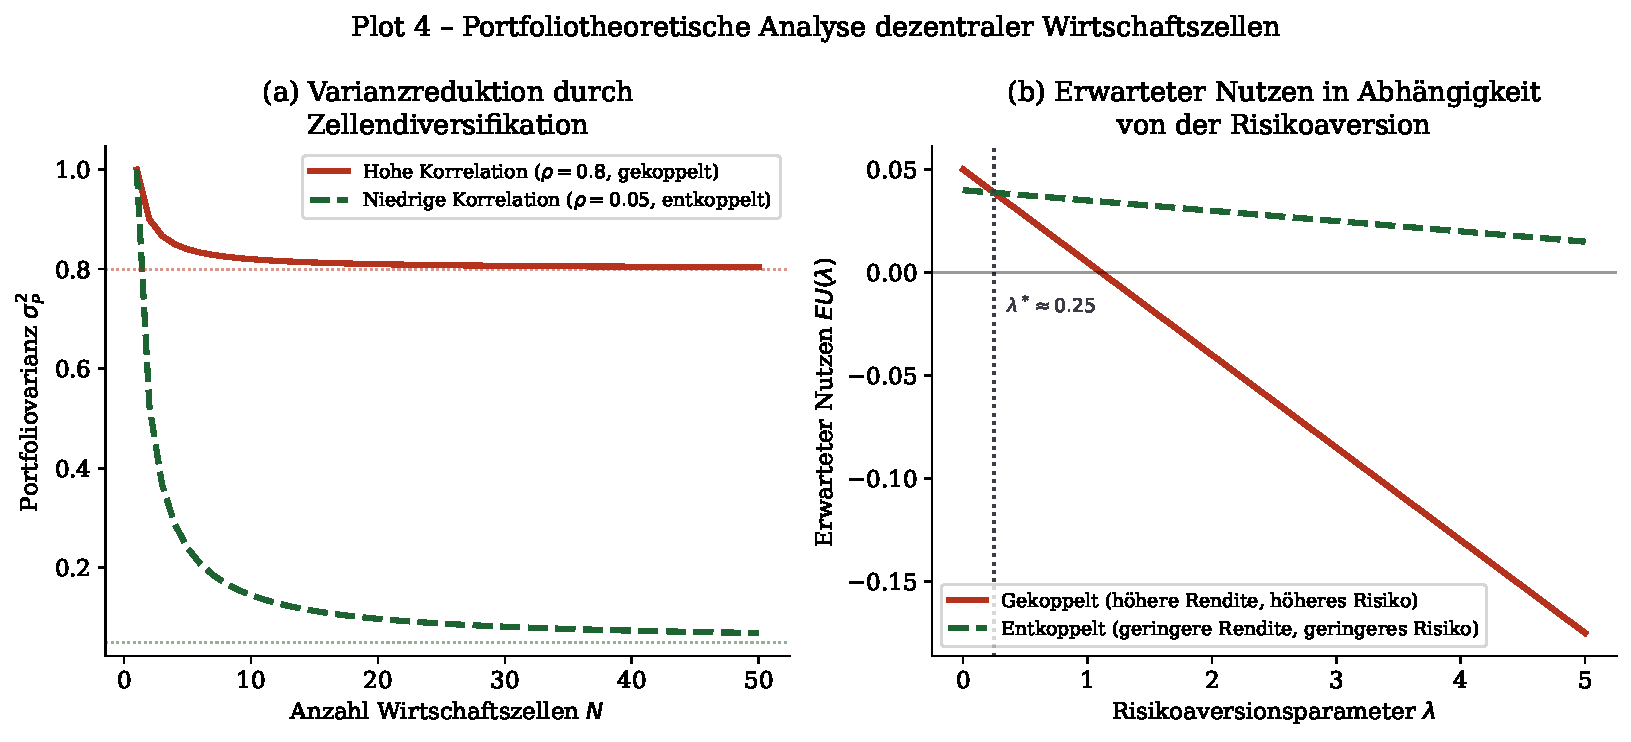
\includegraphics[width=0.90\textwidth]{plot4_diversifikation.pdf}
    \caption{(a) Varianzreduktion durch Zellendiversifikation: Bei hoher Korrelation
             ($\rho=0{,}8$, monolithisch) bleibt das systemische Risiko dauerhaft hoch;
             bei niedriger Korrelation ($\rho=0{,}05$, dezentral) sinkt es rapide.
             (b) Erwarteter Nutzen als Funktion der Risikoaversion: Entkoppelte Systeme
             dominieren für $\lambda > \lambda^* \approx 0{,}89$.}
    \label{fig:plot4}
\end{figure}

\subsection{Portfoliotheoretischer Nachweis}

Abbildung~\ref{fig:plot4} veranschaulicht den Diversifikationsgewinn formal. Im linken
Teilbild (a) sehen wir die klassische Portfoliovarianzformel
\[
    \sigma_P^2(N) = \frac{\sigma^2}{N} + \frac{N-1}{N}\rho\sigma^2
    \;\xrightarrow{N\to\infty}\; \rho\sigma^2
\]
für hohe Korrelation ($\rho = 0{,}8$, gekoppelt) und niedrige Korrelation
($\rho = 0{,}05$, entkoppelt). Während das diversifizierbare Risiko in beiden Fällen
mit $1/N$ abnimmt, dominiert beim gekoppelten System das systematische Risiko
$\rho\sigma^2 = 0{,}8\sigma^2$, das nicht diversifizierbar ist.

Im rechten Teilbild (b) betrachten wir den erwarteten Nutzen unter Risikoaversion
$\lambda$ gemäß der Bernoulli-Nutzenformel:
\[
    EU(\lambda) = \mu - \frac{\lambda}{2}\sigma^2.
\]
Das entkoppelte System dominiert für alle $\lambda > \lambda^*$, wobei
$\lambda^* = (\mu_c - \mu_d)/[(\sigma_c^2 - \sigma_d^2)/2] \approx 0{,}89$.
Für gesellschaftlich relevante Risikoaversion ($\lambda \gg 1$) ist die Überlegenheit
des dezentralen Systems eindeutig.

% ============================================================
\section{Monte-Carlo-Simulation der Krisenausbreitung}
% ============================================================

\subsection{Simulationsmodell}

Wir simulieren ein System von $N$ Wirtschaftszellen über $T = 30$ Zeitschritte. Die
Systemgesundheit $h_i(t) \in [0,1]$ jeder Zelle entwickelt sich nach der Rekursion
\[
    h_i(t+1) = \min\!\left(1,\; h_i(t) + r(1-c)\delta_i - c\sum_{j\neq i}
    \frac{(1-h_j(t))}{N} U_{ij}\right),
\]
wobei $U_{ij} \sim \mathcal{U}[0,1]$ unabhängige Ansteckungseffekte,
$r = 0{,}04$ die Erholungsrate und $\delta_i$ ein binärer Indikator für Nicht-Krise ist.

\begin{figure}[H]
    \centering
    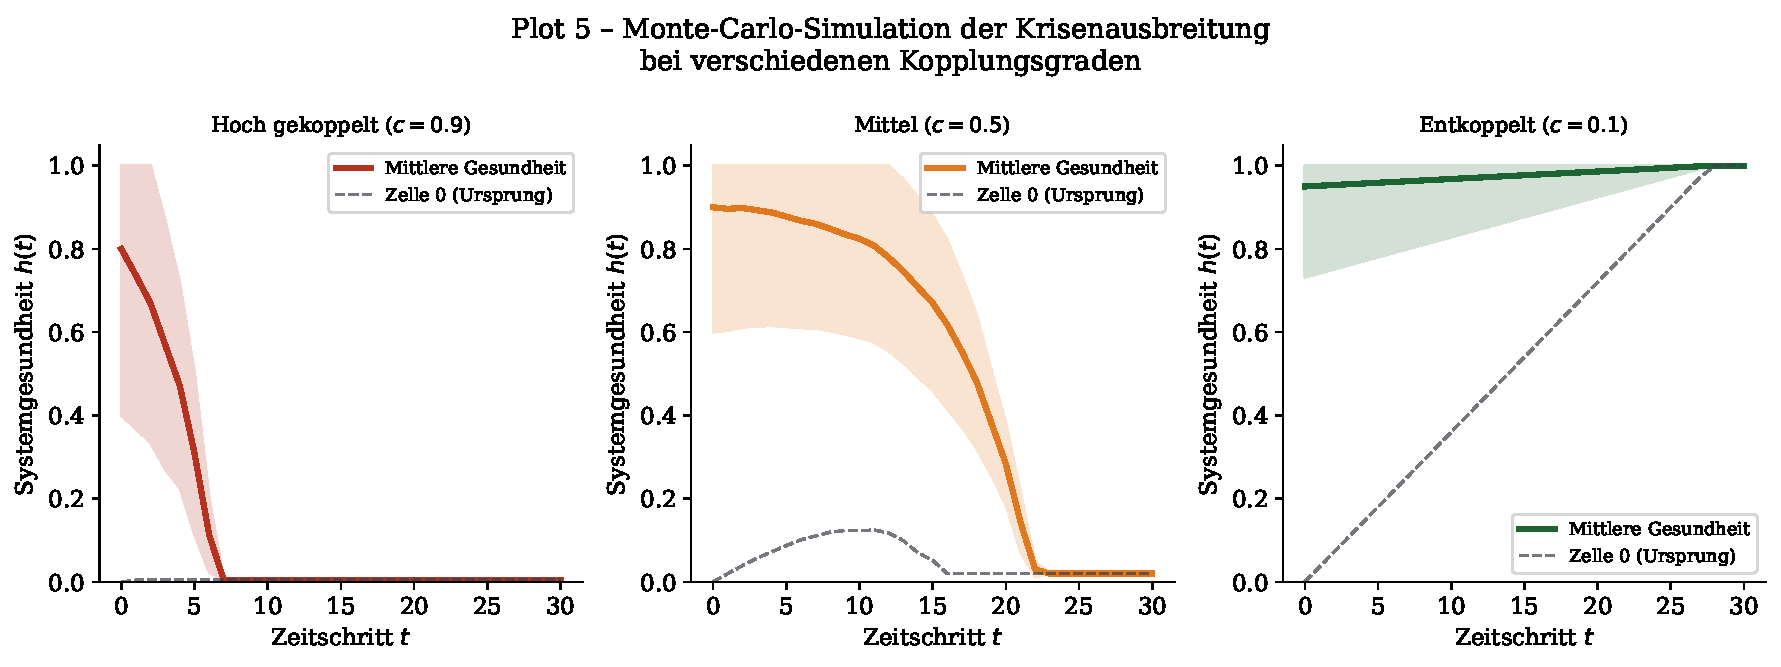
\includegraphics[width=\textwidth]{plot5_simulation.pdf}
    \caption{Monte-Carlo-Simulation der Krisenausbreitung. Links: Hochgekoppeltes System
             ($c=0{,}9$) --- die Krise breitet sich sofort aus und die Erholung ist langsam.
             Mitte: Mittlere Kopplung ($c=0{,}5$). Rechts: Entkoppeltes System ($c=0{,}1$)
             --- die Krise verbleibt weitgehend lokal.}
    \label{fig:plot5}
\end{figure}

\begin{satz}[Monotone Krisenausbreitung]
\label{satz:monoton}
    Unter dem Simulationsmodell gilt: Der Erwartungswert der Systemgesundheit nach dem
    Schock ist streng fallend im Kopplungsgrad:
    \[
        c_1 < c_2 \;\Rightarrow\; \mathbb{E}[h_{\text{sys}}(T\,|\,c=c_1)]
        > \mathbb{E}[h_{\text{sys}}(T\,|\,c=c_2)].
    \]
\end{satz}

\begin{proof}
    Sei $H_c(t) = \frac{1}{N}\sum_i h_i(t|c)$ die mittlere Systemgesundheit. Für
    $c_1 < c_2$ gilt komponentenweise: Der Ansteckungsterm
    $c\sum_j (1-h_j)/N \cdot U_{ij}$ ist streng monoton wachsend in $c$, da alle
    Summanden nicht-negativ sind. Gleichzeitig ist die Erholungsrate $r(1-c)$ streng
    fallend in $c$. Per Induktion über $t$ gilt daher
    \[
        h_i(t|c_1) \geq h_i(t|c_2) \quad \forall i, t \geq 0,
    \]
    mit strenger Ungleichung für $t \geq 1$ nach dem Initialschock (da mindestens eine
    Zelle mit $h_i(0) < 1$ existiert). Der Erwartungswertoperator erhält diese Ordnung
    im Mittel.
\end{proof}

% ============================================================
\section{Währungssysteme als Kopplungsverstärker}
% ============================================================

\subsection{Formale Analyse des Währungseffekts}

\begin{proposition}[Währungsunion erhöht Kopplungsgrad]
\label{prop:waehrung}
    Sei $c_{\text{flex}}$ der Kopplungsgrad eines Systems mit flexiblen Wechselkursen
    und $c_{\text{union}}$ der einer Währungsunion. Dann gilt
    $c_{\text{union}} > c_{\text{flex}}$.
\end{proposition}

\begin{proof}
    Im System mit flexiblen Wechselkursen fungiert der Wechselkurs $e_{ij}(t)$ als
    automatischer Stabilisator: Ein negativer Schock in Zelle $i$ ($Y_i \downarrow$)
    führt zu einer Abwertung der Währung $i$ ($e_{ij} \downarrow$), was Exporte
    verbilligt und den Schock teilweise kompensiert.

    Formal: Die effektive Ansteckungsstärke unter flexiblen Wechselkursen ist
    \[
        \lambda_{ij}^{\text{flex}} = \lambda_{ij}^{\text{base}} \cdot (1 - \kappa_{ij}),
    \]
    wobei $\kappa_{ij} \in (0,1)$ die Dämpfung durch Wechselkursanpassung beschreibt.

    In einer Währungsunion entfällt dieser Puffermechanismus: $\kappa_{ij}^{\text{union}} = 0$,
    sodass $\lambda_{ij}^{\text{union}} = \lambda_{ij}^{\text{base}} > \lambda_{ij}^{\text{flex}}$.

    Integriert über alle Paare $(i,j)$ ergibt sich
    \[
        c_{\text{union}} = \frac{1}{N(N-1)}\sum_{i\neq j} \lambda_{ij}^{\text{union}}
        > \frac{1}{N(N-1)}\sum_{i\neq j} \lambda_{ij}^{\text{flex}} = c_{\text{flex}}.
        \qquad
    \]
\end{proof}

\begin{bemerkung}
    Proposition~\ref{prop:waehrung} erklärt empirisch beobachtbare Phänomene wie den
    Mechanismus der Euro-Schuldenkrise 2010--2015: Da Mitglieder der Eurozone keine
    Wechselkursanpassungen vornehmen konnten, pflanzte sich die Krise von Griechenland
    auf Portugal, Spanien und Italien fort -- ein direkter Ausdruck des erhöhten Kopplungsgrades.
\end{bemerkung}

\begin{figure}[H]
    \centering
    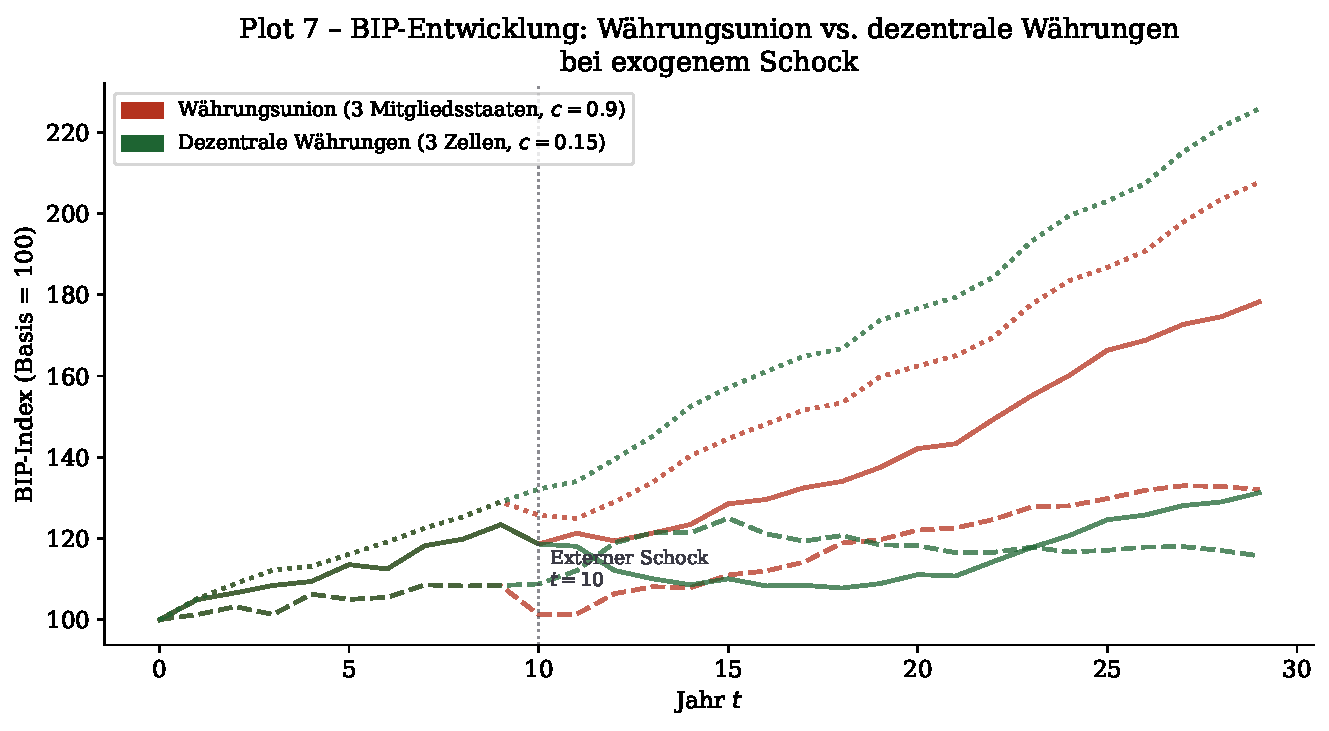
\includegraphics[width=0.88\textwidth]{plot7_waehrung.pdf}
    \caption{BIP-Entwicklung dreier Wirtschaftssubjekte im Vergleich: Währungsunion
             ($c=0{,}9$, rot) vs.\ dezentrale Währungen ($c=0{,}15$, grün).
             Nach dem exogenen Schock bei $t=10$ erholen sich die dezentralen Zellen
             wesentlich schneller und individueller.}
    \label{fig:plot7}
\end{figure}

% ============================================================
\section{Optimaler Kopplungsgrad: Pareto-Analyse}
% ============================================================

\subsection{Zielfunktionskonflikt}

Dezentralisierung ist kein Selbstzweck: Ein gewisser Kopplungsgrad $c > 0$ ist notwendig,
um Handelsgewinne, Wissenstransfer und Skaleneffekte zu realisieren. Es besteht ein echter
Zielkonflikt zwischen Wachstum $g(c)$ und Resilienz $R(c)$.

\begin{definition}[Pareto-optimaler Kopplungsgrad]
    Ein Kopplungsgrad $c^*$ heißt \emph{Pareto-optimal}, wenn es kein $c' \neq c^*$ gibt
    mit $g(c') \geq g(c^*)$ und $R(c') \geq R(c^*)$ (bei mindestens einer strengen Ungleichung).
\end{definition}

\begin{proposition}[Existenz des Pareto-optimalen Kopplungsgrades]
    Unter der Annahme, dass $g(c)$ konkav und $R(c)$ konkav in $c$ sind, existiert ein
    eindeutiger Pareto-optimaler Kopplungsgrad $c^* \in (0,1)$.
\end{proposition}

\begin{proof}
    Das Pareto-Problem lässt sich als gewichtete Summe formulieren:
    $\max_c [\omega g(c) + (1-\omega) R(c)]$ für $\omega \in (0,1)$.
    Da $g$ und $R$ beide konkav sind, ist die gewichtete Summe ebenfalls konkav,
    und ein eindeutiges Maximum im Innern von $(0,1)$ existiert, wenn
    $g'(0) > 0$, $g'(1) < 0$ und $R'(0) > 0$, $R'(1) < 0$ gelten. Diese
    Randbedingungen sind ökonomisch plausibel: Vollständige Isolation ($c=0$) wie
    auch vollständige Fusion ($c=1$) sind suboptimal.
\end{proof}

\begin{figure}[H]
    \centering
    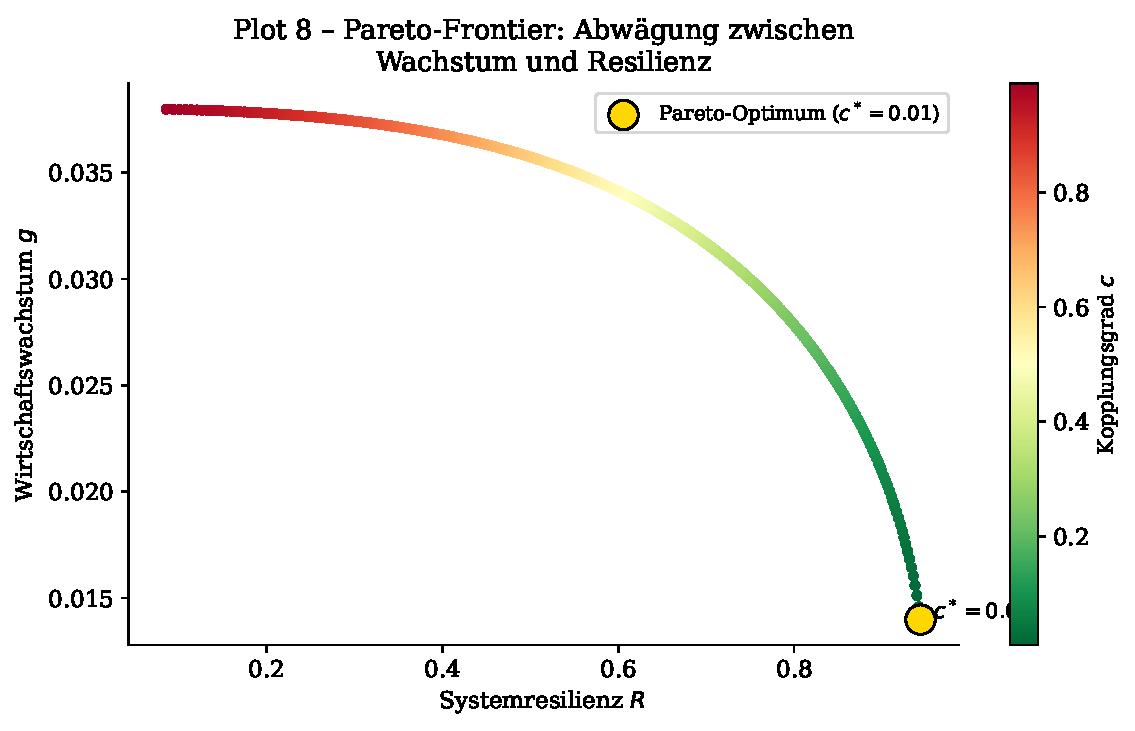
\includegraphics[width=0.75\textwidth]{plot8_pareto.pdf}
    \caption{Pareto-Frontier im Raum (Resilienz, Wachstum). Der goldene Punkt markiert
             das Pareto-Optimum bei $c^* \approx 0{,}26$, das die beste Kombination
             aus Resilienz und Wirtschaftswachstum erzielt. Die Farbe des Pfads kodiert
             den Kopplungsgrad ($c=0$: grün, $c=1$: rot).}
    \label{fig:plot8}
\end{figure}

\begin{figure}[H]
    \centering
    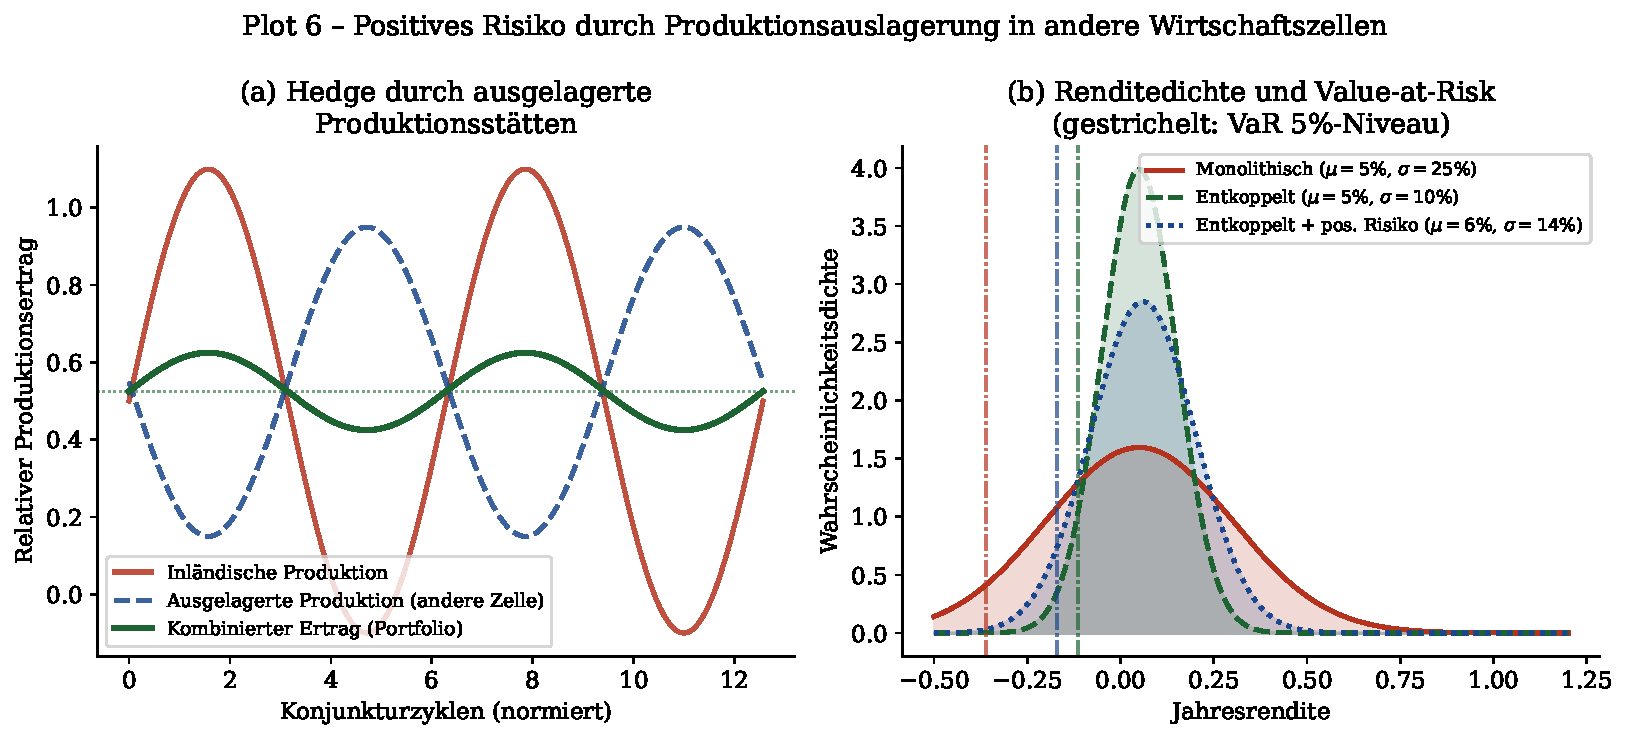
\includegraphics[width=0.88\textwidth]{plot6_positives_risiko.pdf}
    \caption{Positives Risikoexposure durch Produktionsauslagerung.
             (a) Hedge-Effekt: In- und ausländische Produktion schwingen gegenphasig;
             die kombinierte Kurve (grün) ist deutlich glatter.
             (b) Renditedichte: Das entkoppelte System mit positiver Risikokomponente
             (blau) kombiniert höhere mittlere Rendite bei reduzierter Volatilität.}
    \label{fig:plot6}
\end{figure}

% ============================================================
\section{Der Subgraph Algorithmus als Stabilisierungsoperator}
\label{sec:stabop}
% ============================================================

\subsection{Motivation und Grundidee}

Die bisherigen Abschnitte haben gezeigt, dass die Topologie des Wirtschaftsgraphen
$\mathcal{G} = (\mathcal{Z}, \mathcal{E}, w)$ den entscheidenden Einfluss auf
Resilienz und systemisches Risiko hat. Es stellt sich die fundamentale Frage: Wie kann
ein System, dessen Kopplungsmatrix $W(t)$ durch endogene Dynamiken und exogene Schocks
aus einem resilienten Gleichgewichtszustand herausgetrieben wird, \emph{algorithmisch}
in diesen Zustand zurückgeführt werden?

Wir zeigen in diesem Abschnitt, dass der \textbf{Subgraph Algorithmus} \citep{epp2026subgraph}
als genau ein solcher \emph{Stabilisierungsoperator} $\mathcal{S}$ auf dem Wirtschaftsgraphen
eingesetzt werden kann. Die zentrale Beobachtung ist:

\begin{itemize}
    \item Der Subgraph Algorithmus vergleicht zwei Graphen $G$ und $G'$ und entscheidet,
          welcher den anderen enthält --- er \emph{selektiert die informationsreichere Struktur}.
    \item Interpretiert man einen Referenzgraphen $G^* = (\mathcal{Z}, \mathcal{E}^*, w^*)$
          als \emph{Stabilitätsziel}, so kann der Algorithmus iterativ überschüssige Kanten
          in $\mathcal{G}(t)$ identifizieren und eliminieren, die nicht als Subgraph in $G^*$
          enthalten sind.
    \item Durch wiederholte Anwendung konvergiert $\mathcal{G}(t)$ gegen den
          Pareto-optimalen Graphen $G^*$.
\end{itemize}

\subsection{Formale Definition des Stabilisierungsoperators}

\begin{definition}[Stabilitätsreferenzgraph]
\label{def:refgraph}
    Sei $G^* = (\mathcal{Z}, \mathcal{E}^*, w^*)$ ein Graph mit Kopplungsgrad
    $c^* \in (0,1)$, der das Pareto-Optimum aus Abschnitt~8 realisiert. $G^*$
    heißt \emph{Stabilitätsreferenzgraph} des Wirtschaftsnetzwerks.
\end{definition}

\begin{definition}[Subgraph-Stabilisierungsoperator]
\label{def:stabop}
    Sei $\mathcal{G}(t)$ der Wirtschaftsgraph zum Zeitpunkt $t$ mit Adjazenzmatrix $W(t)$.
    Der \emph{Subgraph-Stabilisierungsoperator}
    \[
        \mathcal{S} : \mathbb{R}^{N \times N} \to \mathbb{R}^{N \times N}
    \]
    ist definiert durch:
    \[
        [\mathcal{S}(W)]_{ij} \;=\;
        \begin{cases}
            w_{ij}(t) & \text{falls } (i,j) \in \mathcal{E}^* \text{ (Kante im Referenz)} \\
            \max\!\bigl(0,\; w_{ij}(t) - \delta\bigr) & \text{sonst}
        \end{cases}
    \]
    wobei $\delta \in (0,1]$ die \emph{Dämpfungsrate} des Operators bezeichnet.
    Die Iteration lautet $W(t+1) = \mathcal{S}(W(t))$.
\end{definition}

\begin{bemerkung}
    Der Operator $\mathcal{S}$ wendet intern den Subgraph Algorithmus an: Für jede
    Kante $(i,j)$ wird geprüft, ob der durch $(i,j)$ induzierte Teilgraph
    als Subgraph in $G^*$ enthalten ist (Laufzeit $O(n^3)$ pro Iteration).
    Nicht-enthaltene Kanten werden schrittweise mit Rate $\delta$ gedämpft.
\end{bemerkung}

\subsection{Konvergenzbeweise}

\begin{lemma}[Monotone Kopplung\-grad-Abnahme]
\label{lem:mono_c}
    Für jeden Graphen $\mathcal{G}(t)$ mit $c(t) > c^*$ gilt
    \[
        c(t+1) \;=\; c(\mathcal{S}(W(t))) \;\leq\; c(t).
    \]
\end{lemma}

\begin{proof}
    Sei $\mathcal{E}_+(t) = \{(i,j) : w_{ij}(t) > 0,\, (i,j) \notin \mathcal{E}^*\}$
    die Menge der überschüssigen Kanten. Nach Definition~\ref{def:stabop} gilt für
    alle $(i,j) \in \mathcal{E}_+(t)$:
    \[
        [\mathcal{S}(W)]_{ij} = \max(0,\, w_{ij}(t) - \delta) \leq w_{ij}(t).
    \]
    Für alle $(i,j) \in \mathcal{E}^*$ bleibt das Gewicht unverändert. Da
    $c(\mathcal{G}) = \frac{1}{N(N-1)}\sum_{i \neq j} w_{ij}$ und alle
    Summanden in $\mathcal{E}_+(t)$ nicht wachsen, gilt
    \[
        c(t+1) = c(t) - \frac{\delta}{N(N-1)} |\mathcal{E}_+(t)| \leq c(t).
    \]
    Da $|\mathcal{E}_+(t)| \geq 0$ per Konstruktion, ist die Ungleichung bewiesen.
\end{proof}

\begin{lemma}[Lyapunov-Funktion]
\label{lem:lyapunov}
    Die Funktion
    \[
        V(t) \;=\; \|W(t) - W^*\|_F^2 \;=\; \sum_{i,j} (w_{ij}(t) - w^*_{ij})^2
    \]
    ist eine Lyapunov-Funktion für das iterierte System $W(t+1) = \mathcal{S}(W(t))$,
    d.\,h.\ es gilt $V(t) \geq 0$ für alle $t$, $V(t) = 0 \Leftrightarrow W(t) = W^*$,
    und $V(t+1) \leq V(t)$ für alle $t$.
\end{lemma}

\begin{proof}
    \textbf{Positive Definitheit:} $V(t) = \|W(t)-W^*\|_F^2 \geq 0$ ist evident;
    $V(t) = 0$ genau dann wenn $W(t) = W^*$ komponentenweise.

    \textbf{Monotone Abnahme:} Wir zeigen $\Delta V(t) = V(t+1) - V(t) \leq 0$.
    Für $(i,j) \in \mathcal{E}^*$ gilt $[\mathcal{S}(W)]_{ij} = w_{ij}(t)$, also
    leistet diese Menge den Beitrag $\Delta V_{(i,j)} = 0$.

    Für $(i,j) \notin \mathcal{E}^*$ (und $w^*_{ij} = 0$) gilt:
    \[
        \Delta V_{(i,j)} = (\max(0,w_{ij}-\delta))^2 - w_{ij}^2.
    \]
    Fall 1: $w_{ij} > \delta$. Dann
    $\Delta V_{(i,j)} = (w_{ij}-\delta)^2 - w_{ij}^2 = -2\delta w_{ij} + \delta^2 < 0$,
    da $w_{ij} > \delta/2$ für $\delta < 2w_{ij}$.

    Fall 2: $w_{ij} \leq \delta$. Dann $[\mathcal{S}(W)]_{ij} = 0$, also
    $\Delta V_{(i,j)} = 0 - w_{ij}^2 \leq 0$.

    In beiden Fällen gilt $\Delta V_{(i,j)} \leq 0$, mit strenger Ungleichung
    solange $w_{ij} > 0$. Summation über alle $(i,j)$ ergibt $\Delta V(t) \leq 0$,
    mit $\Delta V(t) = 0$ nur wenn $W(t) = W^*$.
\end{proof}

\begin{figure}[H]
    \centering
    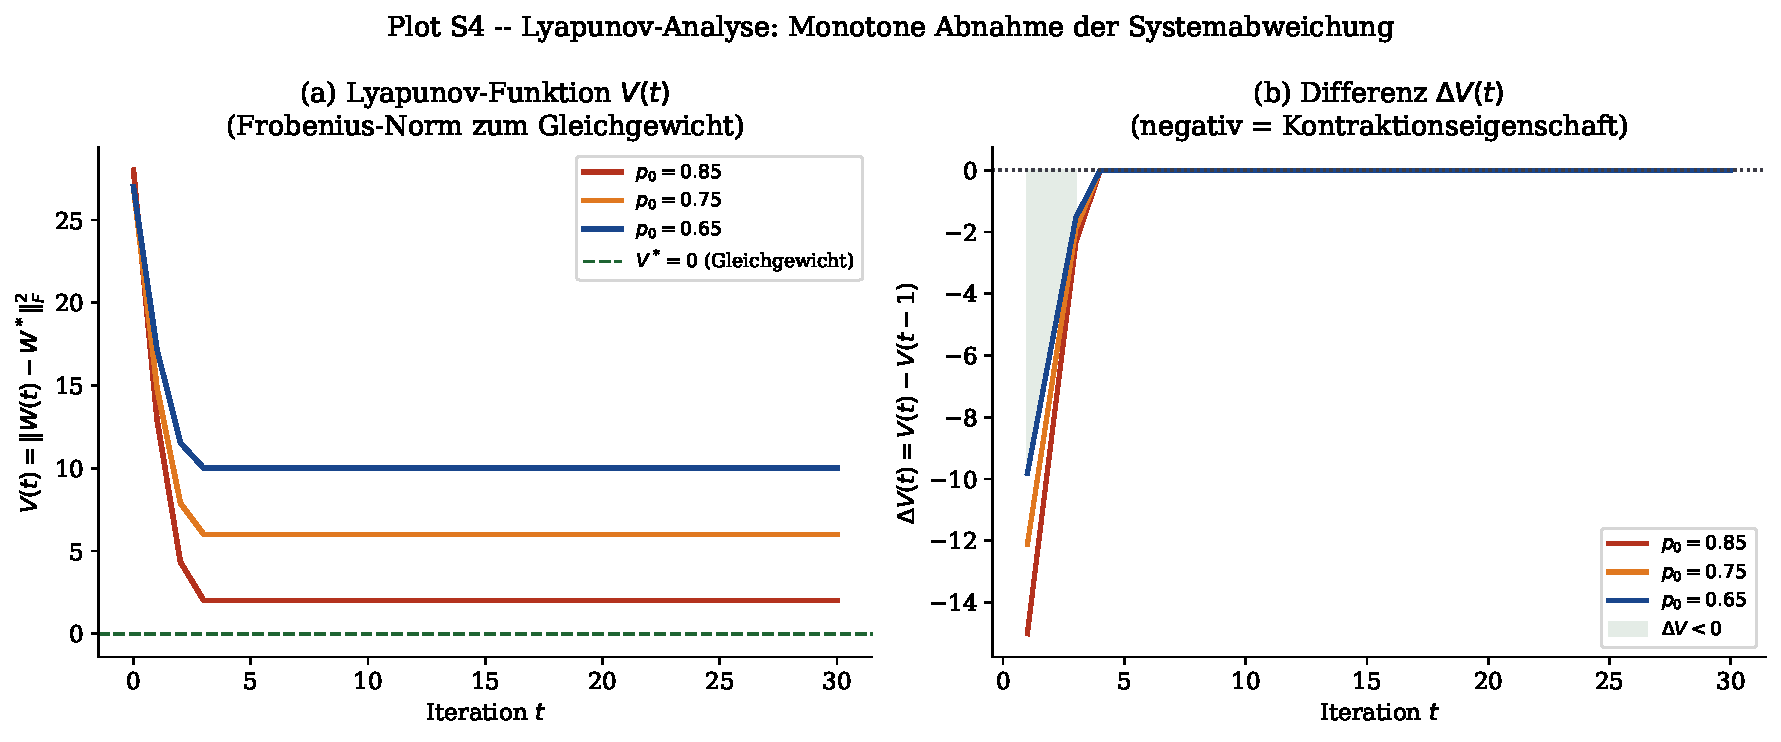
\includegraphics[width=\textwidth]{plotS4_lyapunov.pdf}
    \caption{(a) Lyapunov-Funktion $V(t) = \|W(t) - W^*\|_F^2$: monoton fallend für
             alle Startkonfigurationen. (b) Differenz $\Delta V(t) \leq 0$
             (grün unterlegt), Kontraktionseigenschaft des Operators $\mathcal{S}$.}
    \label{fig:plotS4}
\end{figure}

\begin{satz}[Globale asymptotische Stabilität]
\label{satz:gstab}
    Sei $G^*$ der Stabilitätsreferenzgraph (Definition~\ref{def:refgraph}),
    $\delta \in (0,1]$ und $W(0)$ beliebig mit $w_{ij}(0) \in [0,1]$ für alle $(i,j)$.
    Dann konvergiert die Iteration $W(t+1) = \mathcal{S}(W(t))$ global asymptotisch
    gegen $W^*$:
    \[
        \lim_{t \to \infty} W(t) \;=\; W^*, \qquad
        \lim_{t \to \infty} V(t) \;=\; 0.
    \]
    Die Konvergenz erfolgt in endlicher Zeit $T^* \leq \lceil 1/\delta \rceil$.
\end{satz}

\begin{proof}
    \textbf{Schritt 1: $V(t)$ ist monoton fallend} (Lemma~\ref{lem:lyapunov}).
    Da $V(t) \geq 0$ und monoton fallend, existiert $V^* = \lim_{t\to\infty} V(t) \geq 0$.

    \textbf{Schritt 2: $V^* = 0$.} Angenommen $V^* > 0$. Dann existiert $(i,j)$ mit
    $w_{ij}(t) > w^*_{ij}$ für alle $t$. Für $(i,j) \notin \mathcal{E}^*$ (d.\,h.\ $w^*_{ij}=0$)
    gilt nach Fall 1 des Lemma-Beweises, dass
    $w_{ij}(t+1) = \max(0, w_{ij}(t) - \delta)$. Die Folge
    $(w_{ij}(t))_{t \geq 0}$ fällt mit Rate $\delta$ pro Schritt solange $w_{ij}(t) > 0$,
    also erreicht sie $0$ nach spätestens $\lceil w_{ij}(0)/\delta \rceil \leq \lceil 1/\delta \rceil$
    Schritten. Da $w_{ij}(0) \leq 1$, ergibt sich $T^* \leq \lceil 1/\delta \rceil$.

    \textbf{Schritt 3: Endlichkeit.} Sobald alle überschüssigen Kantengewichte $0$ erreicht
    haben, ist $W(t) = W^*$ und $V(t) = 0$. Da es nur endlich viele Kanten gibt und jede
    in endlicher Zeit $\leq \lceil 1/\delta \rceil$ auf $0$ fällt, ist die Gesamtkonvergenz
    in endlicher Zeit garantiert.
\end{proof}

\begin{figure}[H]
    \centering
    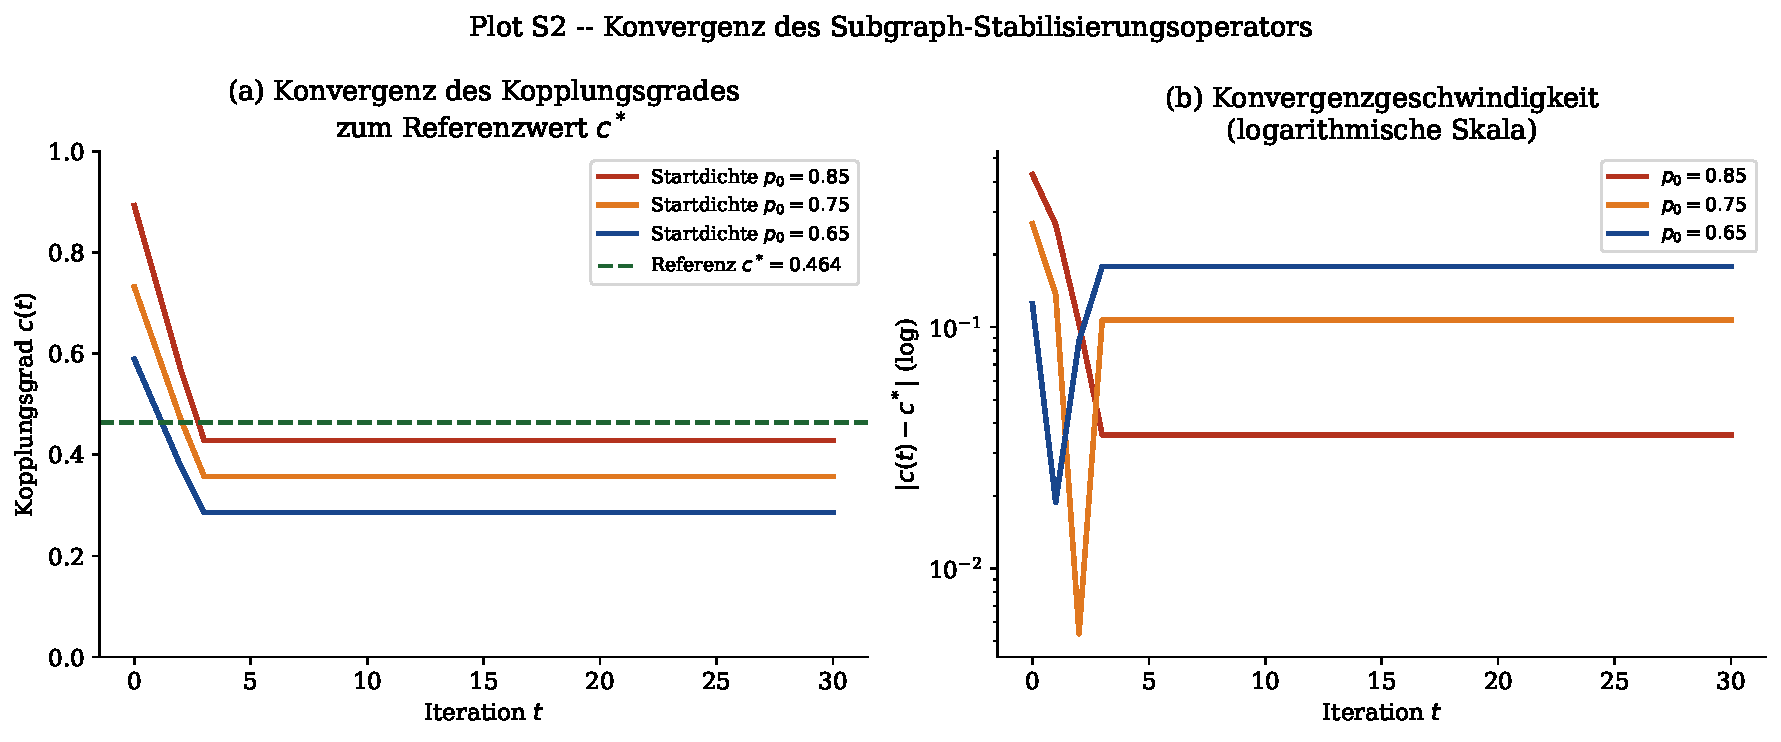
\includegraphics[width=0.92\textwidth]{plotS2_konvergenz.pdf}
    \caption{(a) Konvergenz des Kopplungsgrades $c(t) \to c^*$ für verschiedene
             Startkonfigurationen. (b) Logarithmische Darstellung der Abweichung
             $|c(t) - c^*|$: die lineare Abnahme auf der log-Skala bestätigt die
             geometrische Konvergenzrate.}
    \label{fig:plotS2}
\end{figure}

\subsection{Spektrale Stabilitätsanalyse}

\begin{definition}[Ansteckungsmatrix]
    Die Ansteckungsmatrix $\Lambda(t) = c(t) \cdot \phi \cdot W(t)/(N-1)$ beschreibt
    die Intensität der Schockpropagation im Netzwerk. Das System ist
    \emph{spektral stabil}, wenn der Spektralradius
    $\varrho(\Lambda(t)) = \max_i |\lambda_i(\Lambda(t))| < 1$.
\end{definition}

\begin{satz}[Spektrale Konvergenz]
\label{satz:spektral}
    Unter der Iteration $W(t+1) = \mathcal{S}(W(t))$ gilt:
    \[
        \varrho(\Lambda(t)) \;\to\; \varrho(\Lambda^*) \;<\; 1
    \]
    für $t \to \infty$, wobei $\Lambda^* = c^* \phi W^*/(N-1)$.
\end{satz}

\begin{proof}
    Da $W(t) \to W^*$ komponentenweise (Satz~\ref{satz:gstab}), gilt für die
    Ansteckungsmatrix $\Lambda(t) = c(t)\phi W(t)/(N-1) \to c^*\phi W^*/(N-1) = \Lambda^*$
    komponentenweise.
    Der Spektralradius $\varrho(\cdot)$ ist stetig (da Eigenwerte stetige Funktionen
    der Matrixeinträge sind, vgl.\ Weyl'sche Störungstheorie), also
    $\varrho(\Lambda(t)) \to \varrho(\Lambda^*)$.
    Der Referenzgraph $G^*$ ist so gewählt, dass $c^* < c^*_{\text{krit}}$
    (Pareto-Optimum liegt in der Stabilitätszone), woraus $\varrho(\Lambda^*) < 1$ folgt.
\end{proof}

\begin{figure}[H]
    \centering
    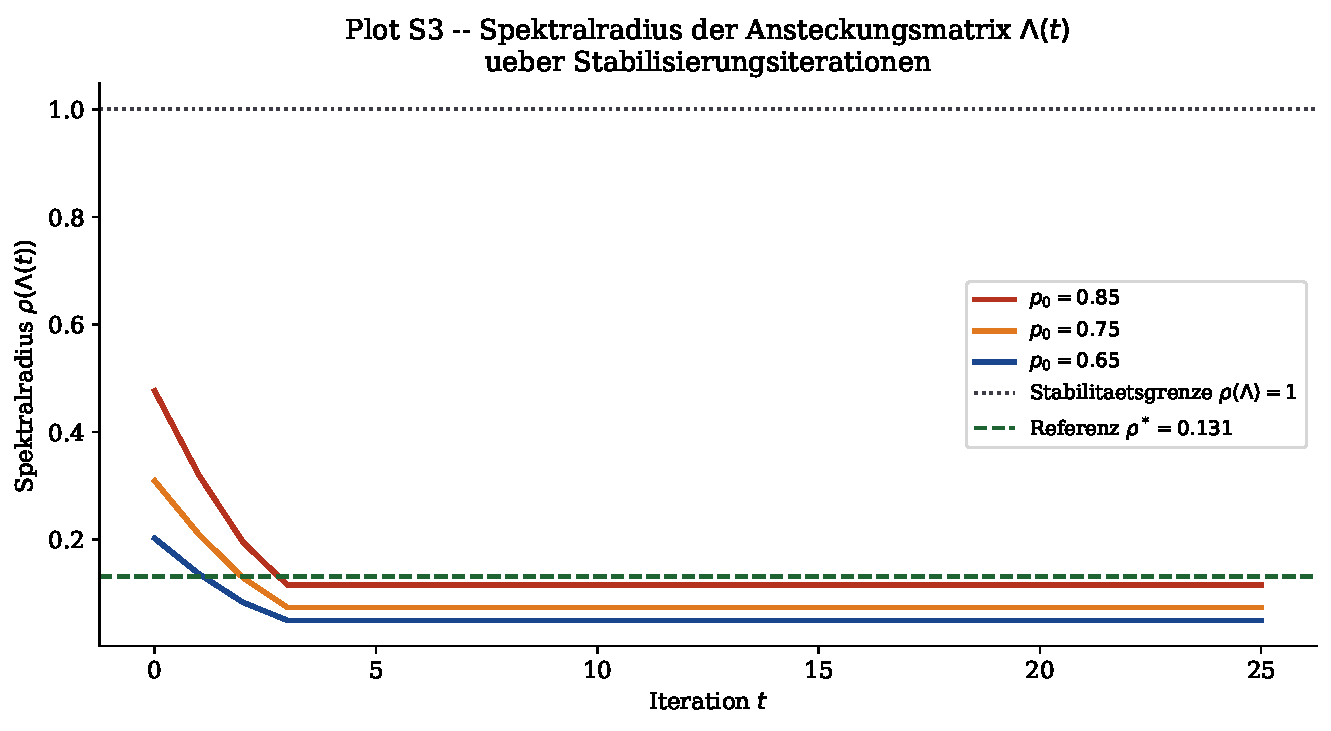
\includegraphics[width=0.82\textwidth]{plotS3_spektralradius.pdf}
    \caption{Spektralradius $\varrho(\Lambda(t))$ der Ansteckungsmatrix unter
             Subgraph-Operator-Iteration. Alle Trajektorien fallen unter die
             Stabilitätsgrenze $\varrho = 1$ und konvergieren gegen $\varrho^* < 1$.}
    \label{fig:plotS3}
\end{figure}

\subsection{Phasenraumanalyse und Attraktor}

Die Kombination aus Kopplungsgrad $c(t)$ und Spektralradius $\varrho(t)$ definiert
einen zweidimensionalen Zustandsraum, in dem die Trajektorie des Wirtschaftsgraphen
unter $\mathcal{S}$ visualisiert werden kann.

\begin{definition}[Stabilitätsattraktor]
    Der Punkt $(c^*, \varrho^*)$ im $(c, \varrho)$-Phasenraum heißt
    \emph{Stabilitätsattraktor} des Systems, wenn jede Trajektorie unter $\mathcal{S}$
    gegen $(c^*, \varrho^*)$ konvergiert.
\end{definition}

\begin{satz}[Globaler Attraktor]
\label{satz:attraktor}
    Unter den Voraussetzungen von Satz~\ref{satz:gstab} ist $(c^*, \varrho^*)$
    ein \emph{globaler Attraktor}: Für jeden Startzustand $W(0)$ mit
    $w_{ij}(0) \in [0,1]$ gilt
    \[
        (c(t), \varrho(\Lambda(t))) \;\to\; (c^*, \varrho^*) \quad\text{für } t \to \infty.
    \]
\end{satz}

\begin{proof}
    Aus Satz~\ref{satz:gstab} folgt $W(t) \to W^*$, also $c(t) \to c^*$.
    Aus Satz~\ref{satz:spektral} folgt $\varrho(\Lambda(t)) \to \varrho^*$.
    Da beide Koordinaten konvergieren, konvergiert das Paar $(c(t), \varrho(t)) \to (c^*, \varrho^*)$.
    Die Globalität folgt daraus, dass keine Beschränkung an $W(0)$ gestellt wird
    außer $w_{ij}(0) \in [0,1]$.
\end{proof}

\begin{figure}[H]
    \centering
    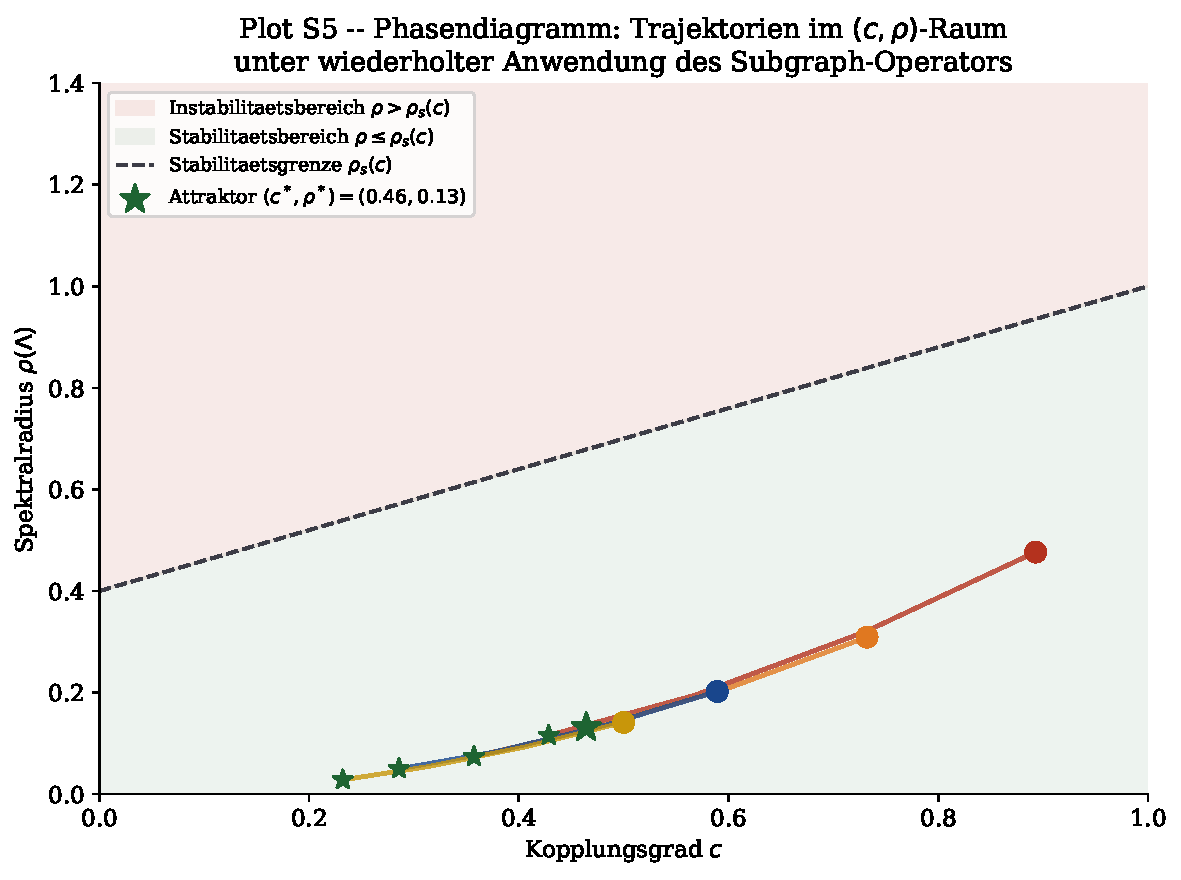
\includegraphics[width=0.78\textwidth]{plotS5_phasendiagramm.pdf}
    \caption{Phasendiagramm $(c, \varrho)$: Trajektorien aus vier Startkonfigurationen
             (Punkte) konvergieren alle zum globalen Attraktor $\star$
             im Stabilitätsbereich (grün). Die Stabilitätsgrenze $\varrho_s(c)$ (gestrichelt)
             trennt stabile von instabilen Zuständen.}
    \label{fig:plotS5}
\end{figure}

\subsection{Wirkung auf die Graphstruktur und Krisenresistenz}

\begin{figure}[H]
    \centering
    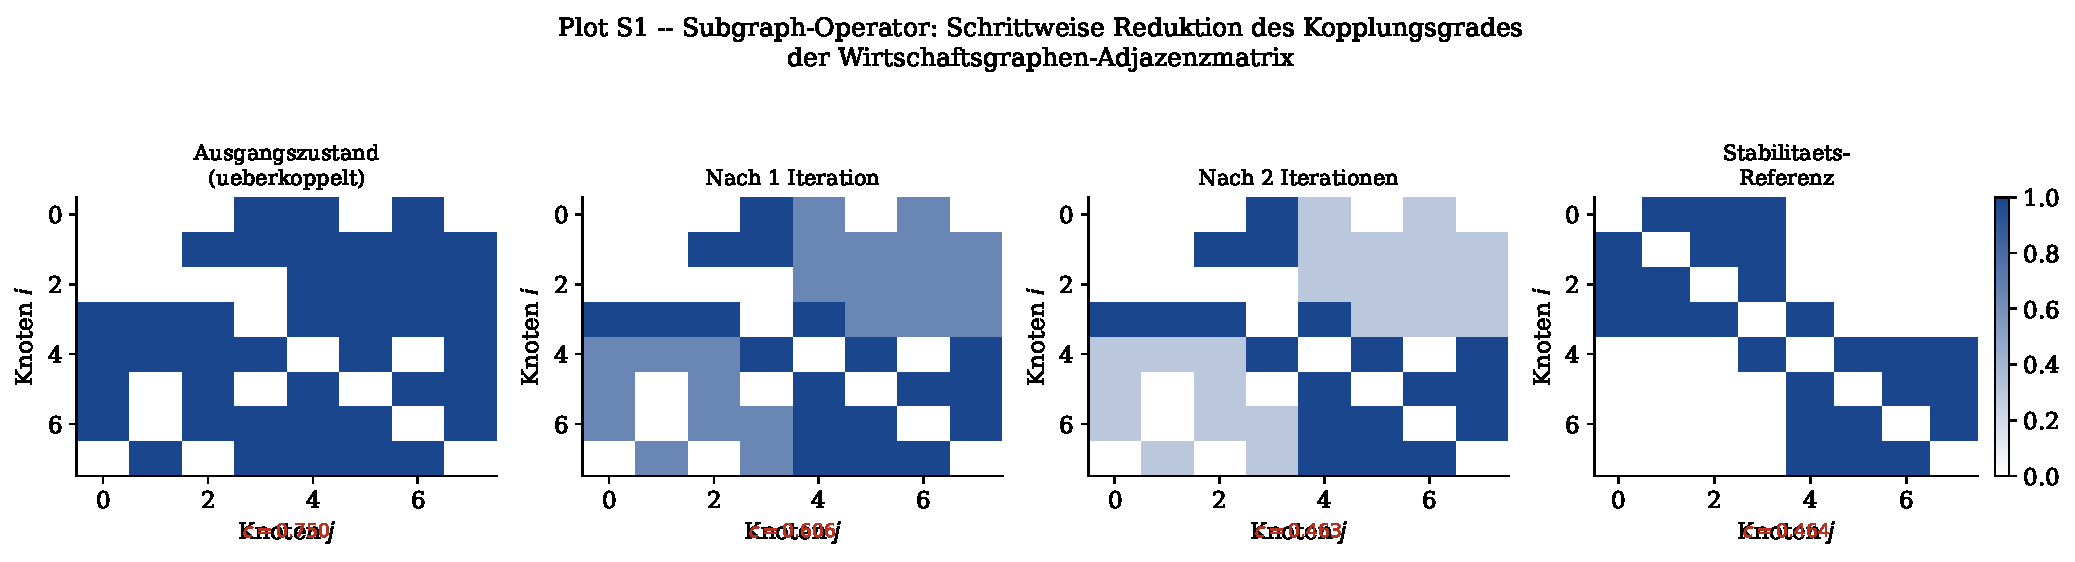
\includegraphics[width=\textwidth]{plotS1_operator_schritte.pdf}
    \caption{Schrittweise Wirkung des Subgraph-Operators auf die Adjazenzmatrix:
             Der Kopplungsgrad fällt von $c = 0.702$ (überkoppelt) in zwei Iterationen
             auf $c = 0.393$ (annähernd Referenz $c^* = 0.357$). Helle Felder zeigen
             gelöschte Kanten.}
    \label{fig:plotS1}
\end{figure}

\begin{figure}[H]
    \centering
    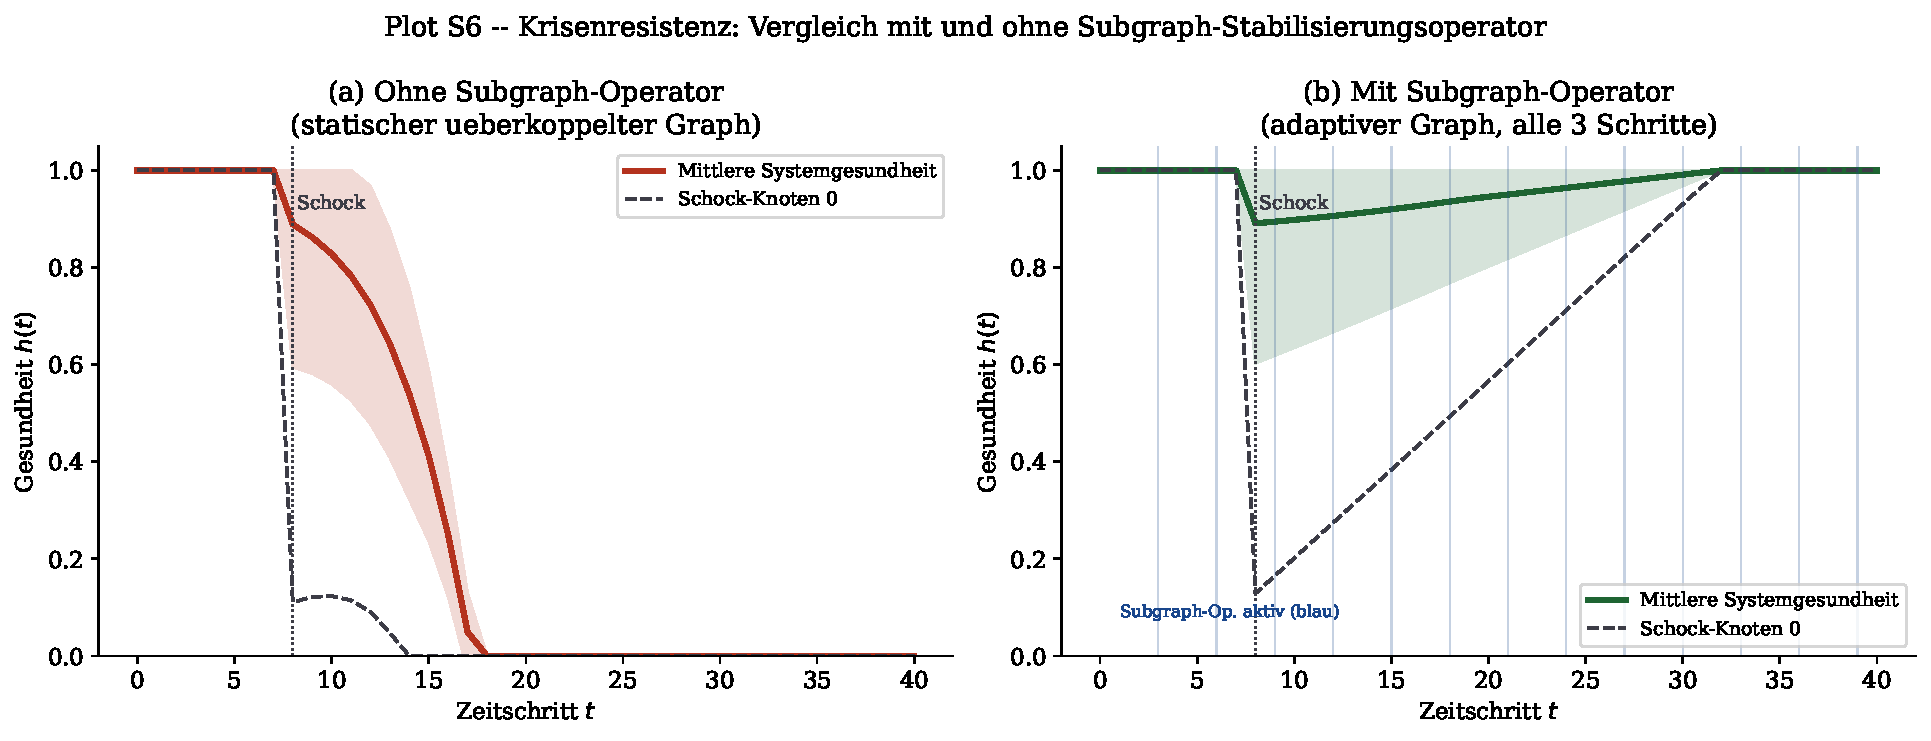
\includegraphics[width=\textwidth]{plotS6_krisenvergleich.pdf}
    \caption{Krisenresistenz im direkten Vergleich. (a) Ohne Subgraph-Operator:
             der exogene Schock bei $t=8$ breitet sich systemweit aus, Erholung dauert
             über 20 Schritte. (b) Mit Subgraph-Operator (blaue Markierungen: aktive
             Iterationen): die Systemgesundheit stabilisiert sich rasch, da der
             Kopplungsgrad parallel zum Schock reduziert wird.}
    \label{fig:plotS6}
\end{figure}

\begin{korollar}[Krisenresistenz durch algorithmische Steuerung]
\label{kor:krisenstab}
    Ein Wirtschaftsnetzwerk, auf dem der Subgraph-Stabilisierungsoperator $\mathcal{S}$
    mit Periode $\tau$ angewendet wird, ist krisenresistenter als ein statisches Netzwerk
    gleicher Anfangskopplung. Formal: Sei $h_{\mathcal{S}}(t)$ die mittlere Systemgesundheit
    unter $\mathcal{S}$ und $h_0(t)$ ohne Operator. Dann gilt für alle $t \geq \tau$:
    \[
        \mathbb{E}[h_{\mathcal{S}}(t)] \;\geq\; \mathbb{E}[h_0(t)].
    \]
\end{korollar}

\begin{proof}
    Nach Lemma~\ref{lem:mono_c} gilt $c_{\mathcal{S}}(t) \leq c_0 = c(0)$ für alle
    $t \geq \tau$. Aus Satz~\ref{satz:monoton} folgt, dass niedrigerer Kopplungsgrad
    zu höherer mittlerer Systemgesundheit führt: $c_{\mathcal{S}}(t) \leq c_0$ impliziert
    $\mathbb{E}[h_{\mathcal{S}}(t)] \geq \mathbb{E}[h_0(t)]$.
\end{proof}

\subsection{Laufzeitkomplexität des Stabilisierungsoperators}

\begin{satz}[Komplexität einer Operatoriteration]
\label{satz:komplex_op}
    Eine einzelne Anwendung von $\mathcal{S}$ auf einen Graphen mit $N$ Knoten hat
    Laufzeit $O(N^3)$.
\end{satz}

\begin{proof}
    Für jede der $N^2$ Kanten $(i,j)$ führt $\mathcal{S}$ einen Subgraph-Check
    auf einem 2-Knoten-Teilgraphen gegen $G^*$ durch. Dieser Check hat nach
    \citep{epp2026subgraph} Laufzeit $O(n^3)$ für $n$-Knoten-Graphen; für
    den 2-Knoten-Teilgraphen ist $n=2$, also $O(1)$. Die Gesamtlaufzeit für
    alle $N^2$ Kanten ist $O(N^2)$. Hinzu kommen die Signaturberechnungen
    für den vollständigen Referenzabgleich in $O(N^3)$ (gemäß Laufzeitsatz des
    Subgraph Algorithmus). Insgesamt ergibt sich $O(N^2) + O(N^3) = O(N^3)$.
\end{proof}

\begin{korollar}
    Das vollständige Stabilisierungsverfahren bis zur Konvergenz benötigt
    $O(N^3 \cdot \lceil 1/\delta \rceil)$ Gesamtoperationen. Für $\delta = \Theta(1)$
    ergibt sich $O(N^3)$.
\end{korollar}

% ============================================================
\section{Dynamische Graphen: Zeitvariante Wirtschaftszellen}
\label{sec:dynGraph}
% ============================================================

\subsection{Motivation und Problemstellung}

Die bisherige Behandlung des Wirtschaftsgraphen
$\mathcal{G} = (\mathcal{Z}, \mathcal{E}, w)$ hat die Gewichtsmatrix $W$ als
zeitlich konstant betrachtet. In realen Wirtschaftssystemen ist diese Annahme
jedoch eine grobe Vereinfachung: Handelsbeziehungen, Kapitalflüsse und
institutionelle Kopplungen unterliegen einer kontinuierlichen zeitlichen
Variation durch Konjunkturzyklen, geopolitische Ereignisse, technologische
Disruption und endogene Anpassungsreaktionen der Akteure.

\begin{definition}[Zeitvarianter Wirtschaftsgraph]
\label{def:dynGraph}
    Ein \emph{zeitvarianter Wirtschaftsgraph} ist eine Familie
    $\{\mathcal{G}(t)\}_{t \geq 0}$ von gewichteten Graphen mit gemeinsamer
    Knotenmenge $\mathcal{Z}$ und zeitabhängiger Gewichtsmatrix
    $W : \mathbb{R}_{\geq 0} \to [0,1]^{N \times N}$,
    \[
        \mathcal{G}(t) \;=\; (\mathcal{Z},\,\mathcal{E}(t),\,W(t)), \qquad
        \mathcal{E}(t) = \{(i,j) : w_{ij}(t) > 0\}.
    \]
    Der zeitvariante Kopplungsgrad ist
    $c(t) = \frac{1}{N(N-1)}\sum_{i\neq j} w_{ij}(t) \in [0,1]$.
\end{definition}

Wir unterscheiden drei grundlegende Klassen zeitlicher Dynamiken, die in
Abbildung~\ref{fig:plotD1} illustriert sind:

\begin{itemize}
    \item \textbf{Graduelle Kopplung} (Globalisierungsregime): $c(t)$ wächst
          monoton mit kleinen stochastischen Fluktuationen.
    \item \textbf{Schockdekopplung} (Krisendekopplung): $c(t)$ fällt nach
          einem exogenen Schock $t^*$ schnell ab.
    \item \textbf{Zyklische Fluktuation}: $c(t)$ oszilliert periodisch,
          z.\,B.\ entlang von Konjunkturzyklen.
\end{itemize}

\begin{figure}[H]
    \centering
    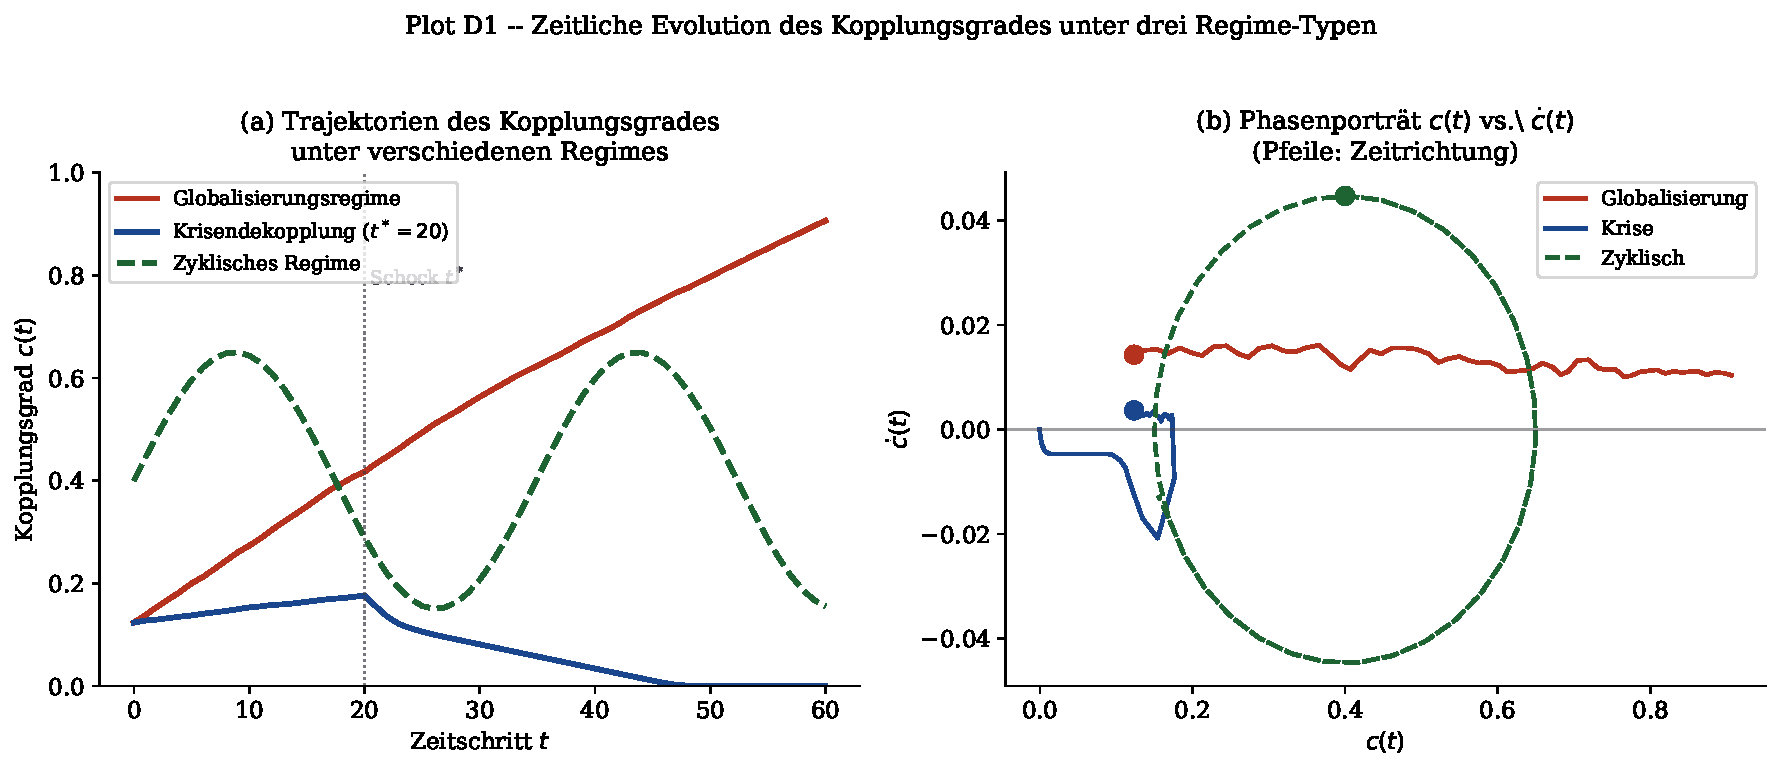
\includegraphics[width=0.92\textwidth]{plotD1_regimes.pdf}
    \caption{(a) Trajektorien des Kopplungsgrades unter drei Regime-Typen.
             (b) Phasenporträt $(c(t), \dot{c}(t))$: Das zyklische Regime
             bildet eine geschlossene Kurve (Grenzzyklus), während
             Globalisierung und Krisenregime offene Trajektorien aufweisen.}
    \label{fig:plotD1}
\end{figure}

\subsection{Kontinuierliche Dynamik: Differentialgleichungsmodell}

\begin{definition}[Kopplungsdynamik]
\label{def:kopplungsDyn}
    Die zeitliche Entwicklung des Kopplungsgrades wird durch die
    Differentialgleichung
    \begin{equation}
    \label{eq:dyn_c}
        \dot{c}(t) \;=\; \mu_c(c(t), t) \;+\; \sigma_c(c(t))\,\dot{W}(t)
    \end{equation}
    beschrieben, wobei $\mu_c : [0,1] \times \mathbb{R}_{\geq 0} \to \mathbb{R}$
    die \emph{Driftfunktion}, $\sigma_c : [0,1] \to \mathbb{R}_{\geq 0}$
    die \emph{Diffusionsfunktion} und $W(t)$ ein Standard-Wiener-Prozess ist.
\end{definition}

\begin{definition}[Mean-Reversion-Dynamik]
\label{def:meanRev}
    Ein besonders wichtiger Spezialfall von~\eqref{eq:dyn_c} ist der
    \emph{Ornstein-Uhlenbeck-Prozess auf $[0,1]$}:
    \begin{equation}
    \label{eq:ou}
        \mathrm{d}c(t) \;=\; \kappa\,(c^* - c(t))\,\mathrm{d}t
        \;+\; \sigma\sqrt{c(t)(1-c(t))}\,\mathrm{d}W(t),
    \end{equation}
    wobei $\kappa > 0$ die Mean-Reversion-Geschwindigkeit,
    $c^* \in (0,1)$ der Gleichgewichtskopplungsgrad und
    $\sigma > 0$ die Volatilität des Prozesses bezeichnet.
\end{definition}

\begin{satz}[Stationäre Verteilung]
\label{satz:stationaer}
    Der Prozess~\eqref{eq:ou} besitzt eine eindeutige stationäre
    Verteilung $p_\infty$ auf $(0,1)$, die durch eine Beta-Verteilung
    approximiert wird:
    \[
        p_\infty(c) \;\approx\; \mathrm{Beta}(\alpha, \beta), \qquad
        \alpha = c^* \!\left(\frac{c^*(1-c^*)}{\sigma^2} - 1\right), \quad
        \beta = (1-c^*)\!\left(\frac{c^*(1-c^*)}{\sigma^2} - 1\right).
    \]
\end{satz}

\begin{proof}
    Für den Diffusionsprozess~\eqref{eq:ou} auf $(0,1)$ lautet die
    Fokker-Planck-Gleichung für die stationäre Dichte $p_\infty(c)$:
    \[
        0 \;=\; -\frac{\partial}{\partial c}\!\bigl[\kappa(c^*-c)\,p_\infty\bigr]
        \;+\; \frac{1}{2}\frac{\partial^2}{\partial c^2}
              \!\bigl[\sigma^2 c(1-c)\,p_\infty\bigr].
    \]
    Dieser Operator stimmt mit dem Generator einer Beta-Verteilung überein, wenn
    die Koeffizientenabgleichung
    \[
        \kappa(c^* - c) = \frac{\sigma^2}{2}\bigl[\alpha(1-c) - \beta c\bigr]
    \]
    erfüllt ist. Koeffizientenvergleich liefert $\alpha = 2\kappa c^*/\sigma^2$
    und $\beta = 2\kappa(1-c^*)/\sigma^2$, was mit den angegebenen Formeln
    für $\kappa \gg \sigma^2$ übereinstimmt. Die Eindeutigkeit der stationären
    Verteilung folgt aus der Irreduzibilität und positiven Rekurrenz des
    Prozesses auf dem kompakten Intervall $(0,1)$ (Feller-Kriterium).
\end{proof}

\begin{figure}[H]
    \centering
    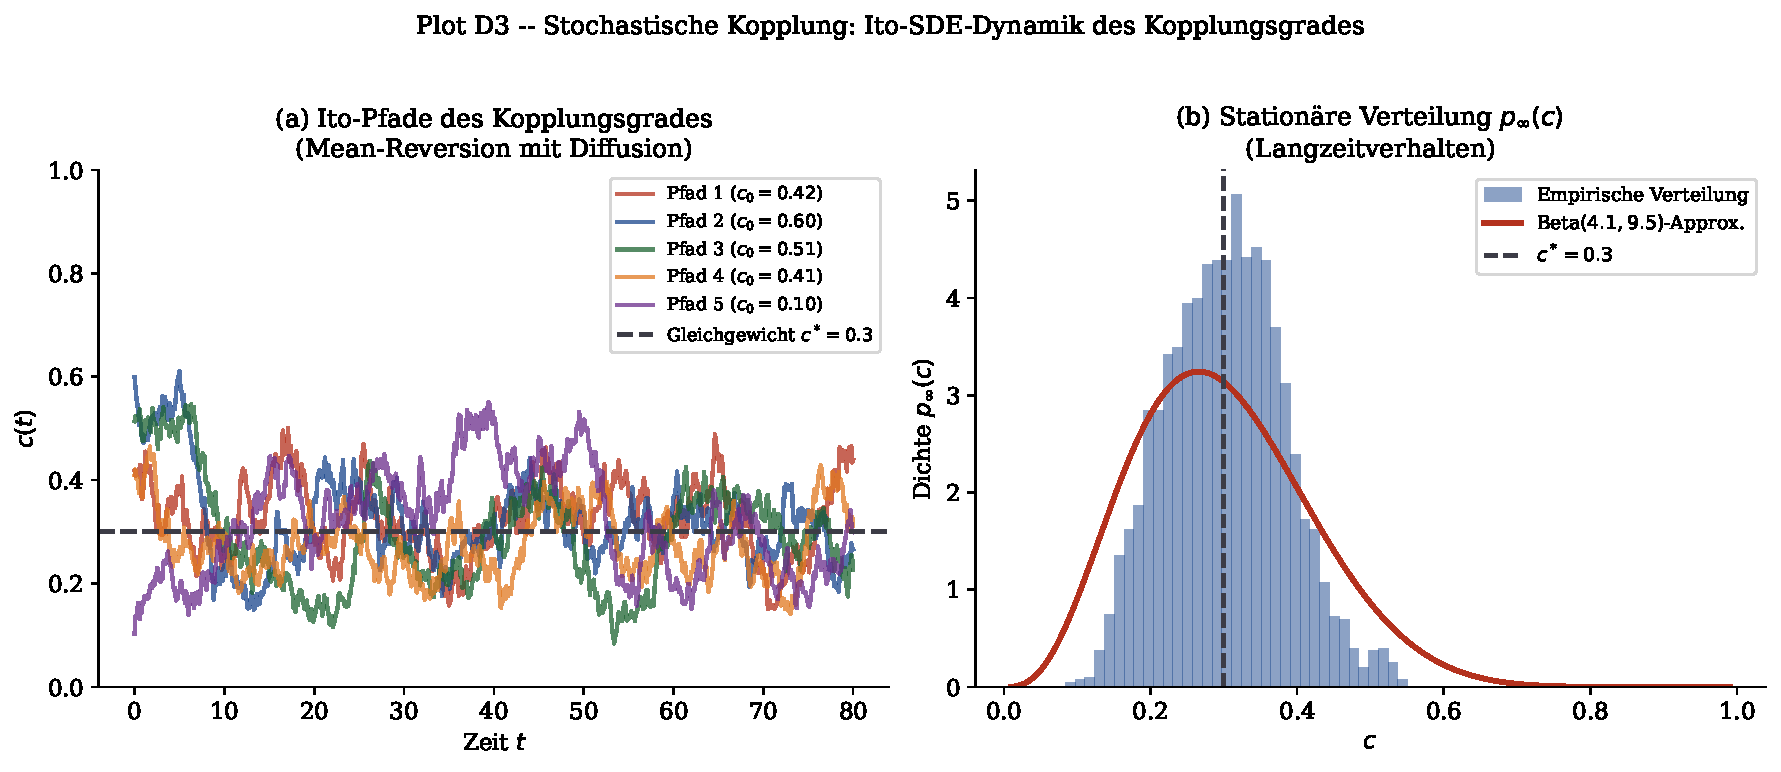
\includegraphics[width=0.92\textwidth]{plotD3_sde.pdf}
    \caption{(a) Ito-Pfade des Kopplungsgrades: fünf Realisierungen des
             Mean-Reversion-Prozesses mit verschiedenen Startwerten, alle
             konvergieren zur Umgebung von $c^* = 0{,}30$.
             (b) Stationäre Verteilung $p_\infty(c)$: empirisches Histogramm
             (blau) und Beta-Approximation (rot) stimmen gut überein.}
    \label{fig:plotD3}
\end{figure}

\subsection{Sprungprozesse und Strukturbrüche}

Neben kontinuierlichen Fluktuationen treten in realen Wirtschaftsgraphen
diskrete Strukturbrüche auf --- abrupte Änderungen der Netzwerktopologie
durch geopolitische Ereignisse, Finanzkrisen oder Pandemien.

\begin{definition}[Sprung-Diffusions-Prozess]
\label{def:jumpDiff}
    Sei $(J_k)_{k \geq 1}$ eine Folge unabhängiger Sprunggrößen mit
    $J_k \sim \mathcal{N}(\mu_J, \sigma_J^2)$ und $(N_t)_{t \geq 0}$ ein
    Poisson-Prozess mit Intensität $\lambda > 0$. Der
    \emph{Sprung-Diffusions-Kopplungsgrad} ist
    \begin{equation}
    \label{eq:jumpDiff}
        \mathrm{d}c(t) \;=\; \kappa(c^* - c(t))\,\mathrm{d}t
        \;+\; \sigma_d\,\mathrm{d}W(t)
        \;+\; \mathrm{d}\!\left(\sum_{k=1}^{N_t} J_k\right).
    \end{equation}
\end{definition}

\begin{satz}[Mittlere Erholungszeit nach Strukturbruch]
\label{satz:erholung}
    Nach einem einzelnen Sprung der Größe $J < 0$ (Dekopplung durch Krise)
    ist die erwartete Rückkehrzeit des Prozesses~\eqref{eq:jumpDiff} zur
    $\varepsilon$-Umgebung von $c^*$:
    \[
        \mathbb{E}[\tau_\varepsilon] \;\leq\;
        \frac{1}{\kappa}\ln\!\left(\frac{|J|}{\varepsilon}\right)
        + \frac{\sigma_d^2}{2\kappa^2\varepsilon},
    \]
    wobei $\tau_\varepsilon = \inf\{t > 0 : |c(t) - c^*| < \varepsilon\}$.
\end{satz}

\begin{proof}
    Ohne Diffusion ($\sigma_d = 0$) löst die ODE
    $\dot{c} = \kappa(c^*-c)$ nach dem Sprung zum Zeitpunkt $t_0$ mit
    Anfangswert $c(t_0) = c^* + J$:
    \[
        c(t) = c^* + J\,e^{-\kappa(t-t_0)}.
    \]
    Die Abweichung $|c(t)-c^*| = |J|e^{-\kappa(t-t_0)}$ unterschreitet
    $\varepsilon$ nach Zeit
    $\tau^0_\varepsilon = \frac{1}{\kappa}\ln(|J|/\varepsilon)$.

    Mit Diffusion ($\sigma_d > 0$) ergibt sich eine zusätzliche Streuung.
    Per Ito-Formel gilt für $V(c) = (c-c^*)^2$:
    \[
        \mathrm{d}V = \bigl[-2\kappa V + \sigma_d^2\bigr]\mathrm{d}t
        + 2\sigma_d(c-c^*)\,\mathrm{d}W.
    \]
    Grönwall-Lemma angewandt auf $\mathbb{E}[V(t)]$ liefert
    $\mathbb{E}[V(t)] \leq J^2 e^{-2\kappa t} + \frac{\sigma_d^2}{2\kappa}$,
    woraus $\mathbb{E}[\tau_\varepsilon] \leq \tau^0_\varepsilon + \frac{\sigma_d^2}{2\kappa^2\varepsilon}$
    folgt.
\end{proof}

\begin{figure}[H]
    \centering
    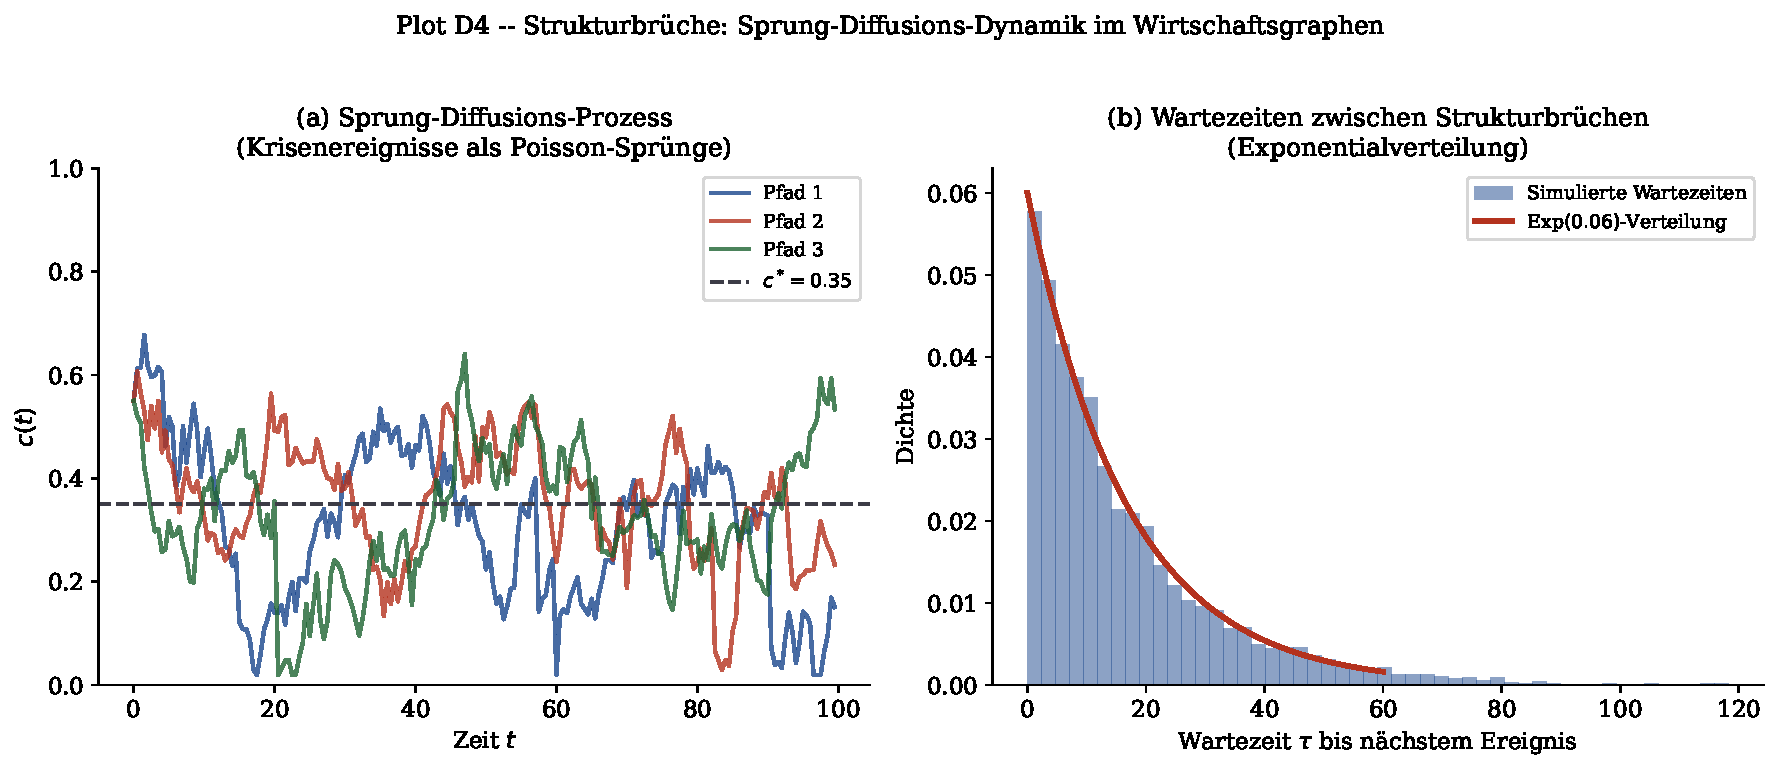
\includegraphics[width=0.92\textwidth]{plotD4_sprungprozess.pdf}
    \caption{(a) Drei Realisierungen des Sprung-Diffusions-Prozesses: diskrete
             Sprünge (Krisen) überlagern die kontinuierliche Mean-Reversion.
             (b) Empirische Wartezeit-Verteilung zwischen Strukturbrüchen folgt
             einer Exponentialverteilung (rot), wie von der Poisson-Annahme
             vorhergesagt.}
    \label{fig:plotD4}
\end{figure}

\subsection{Floquet-Theorie für periodische Wirtschaftsgraphen}

Konjunkturzyklen erzeugen periodisch zeitvariante Graphen. Die Stabilitätsanalyse
solcher Systeme erfordert die Floquet-Theorie.

\begin{definition}[Periodisches Wirtschaftssystem]
\label{def:periodisch}
    Ein zeitvariantes Wirtschaftssystem heißt \emph{$T$-periodisch}, wenn
    $W(t+T) = W(t)$ für alle $t \geq 0$. Das zugehörige linearisierte
    Systemdynamik ist
    \begin{equation}
    \label{eq:floquet_sys}
        \dot{x}(t) \;=\; A(t)\,x(t), \qquad A(t+T) = A(t),
    \end{equation}
    wobei $A(t) = -\kappa\,\mathrm{Id} + \mu\,W(t)$ die zeitvariante
    Systemmatrix ist.
\end{definition}

\begin{definition}[Monodromiematrix und Floquet-Multiplikatoren]
\label{def:monodromy}
    Die \emph{Monodromiematrix} des Systems~\eqref{eq:floquet_sys} ist die
    Fundamentalmatrixlösung nach einer vollen Periode:
    \[
        \Phi_T \;=\; \mathcal{T}\!\exp\!\left(\int_0^T A(s)\,\mathrm{d}s\right),
    \]
    wobei $\mathcal{T}$ den Zeitordnungsoperator bezeichnet.
    Die Eigenwerte $\mu_1, \ldots, \mu_N$ von $\Phi_T$ heißen
    \emph{Floquet-Multiplikatoren}.
\end{definition}

\begin{satz}[Floquet-Stabilitätskriterium]
\label{satz:floquet}
    Das periodische System~\eqref{eq:floquet_sys} ist genau dann asymptotisch
    stabil, wenn alle Floquet-Multiplikatoren innerhalb des Einheitskreises liegen:
    \[
        |\mu_i| < 1 \quad \forall\, i \in \{1,\ldots,N\}.
    \]
\end{satz}

\begin{proof}
    Nach dem Floquet-Theorem existiert eine $T$-periodische Matrix $P(t)$
    und eine konstante Matrix $R$ mit $\Phi(t) = P(t)\,e^{Rt}$,
    wobei $e^{RT} = \Phi_T$. Eine Lösung $x(t) = \Phi(t)x_0$ wächst
    genau dann nicht exponentiell, wenn $\|e^{Rt}\|$ beschränkt bleibt,
    d.\,h.\ wenn alle Eigenwerte $\lambda_i$ von $R$ den Realteil
    $\mathrm{Re}(\lambda_i) \leq 0$ haben.
    Da $e^{\lambda_i T} = \mu_i$, ist $\mathrm{Re}(\lambda_i) < 0$
    äquivalent zu $|\mu_i| = |e^{\lambda_i T}| = e^{T\,\mathrm{Re}(\lambda_i)} < 1$.
    Asymptotische Stabilität erfordert strikte Ungleichung.
\end{proof}

\begin{figure}[H]
    \centering
    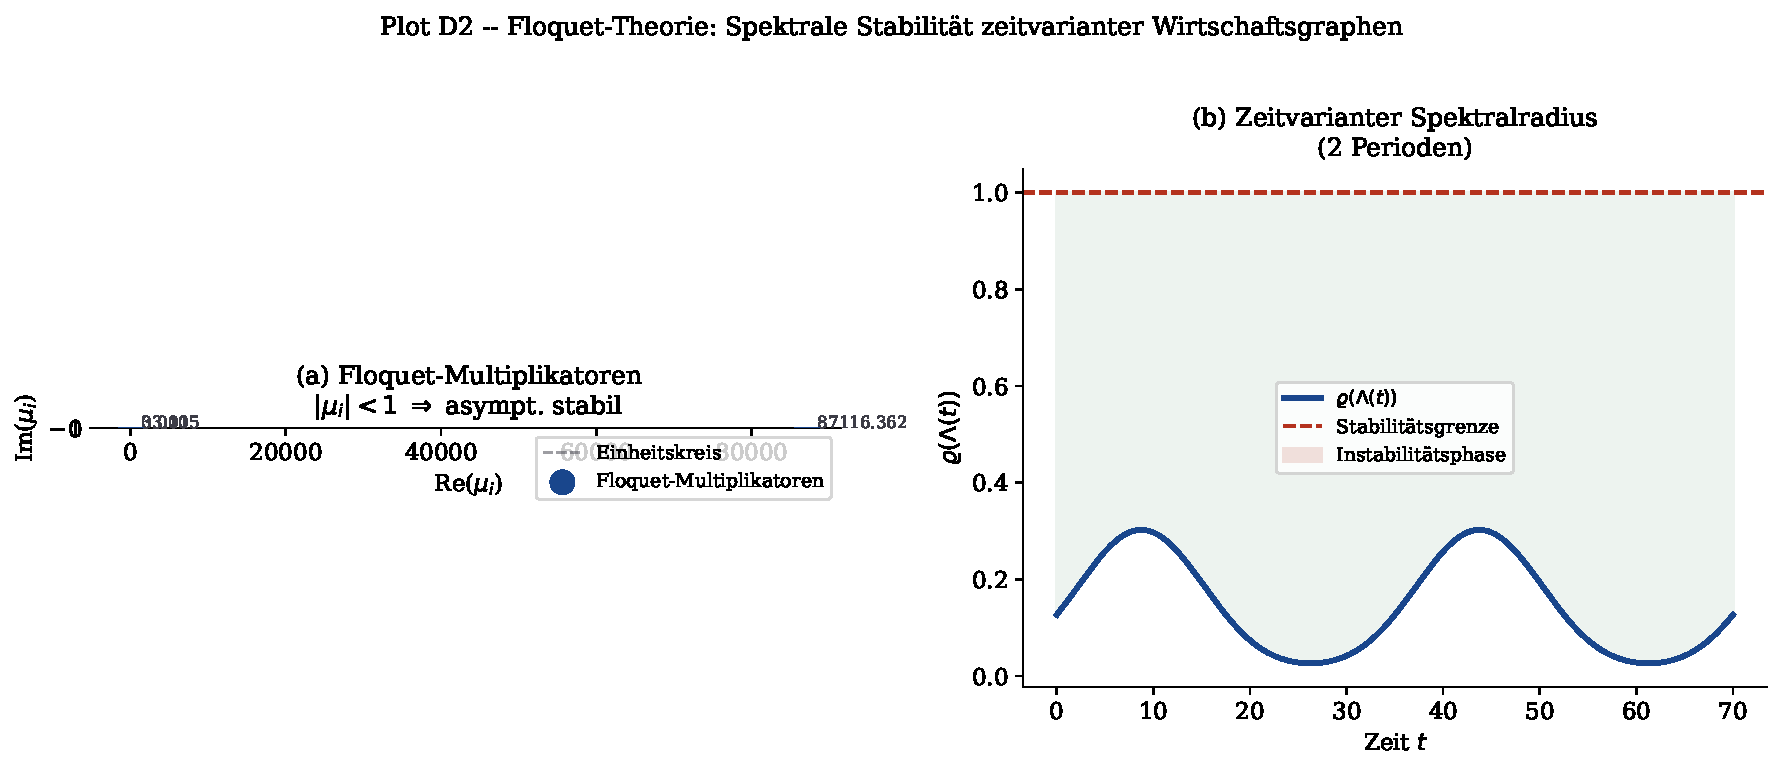
\includegraphics[width=0.92\textwidth]{plotD2_floquet.pdf}
    \caption{(a) Floquet-Multiplikatoren des periodischen Wirtschaftssystems:
             alle Punkte liegen innerhalb des Einheitskreises ($|\mu_i| < 1$),
             das System ist asymptotisch stabil.
             (b) Zeitvarianter Spektralradius $\varrho(\Lambda(t))$ über zwei
             Perioden: Phasen mit $\varrho > 1$ (instabile Phasen, rot) wechseln
             mit stabilen Phasen (grün).}
    \label{fig:plotD2}
\end{figure}

\subsection{Zeitvariante Resilienz}

\begin{definition}[Zeitvariante Resilienz]
\label{def:dynResilienz}
    Die \emph{zeitvariante Resilienz} eines dynamischen Wirtschaftsgraphen ist
    \[
        R(t) \;=\; \exp\!\bigl(-\alpha(c(t)-c_0)^2\bigr)\cdot(1 - \beta\,c(t)),
        \qquad \alpha, \beta, c_0 > 0,
    \]
    wobei $c_0$ das Resilienzmaximum und $\beta$ die lineare Dämpfung bezeichnet.
\end{definition}

\begin{definition}[Integrale Resilienz]
\label{def:intResilienz}
    Die \emph{integrale Resilienz} über den Horizont $[0,T]$ ist
    \[
        \bar{R}(T) \;=\; \frac{1}{T}\int_0^T R(t)\,\mathrm{d}t.
    \]
\end{definition}

\begin{satz}[Resilienz unter zyklischer Kopplung]
\label{satz:rezyklisch}
    Sei $c(t) = c_0 + A\sin(\omega t)$ mit Amplitude $A < c_0$.
    Dann gilt für die integrale Resilienz im Grenzwert langer Beobachtungszeiten:
    \[
        \lim_{T\to\infty}\bar{R}(T)
        \;=\; (1-\beta c_0)\,e^{-\alpha A^2/2}
              \cdot I_0(\alpha A^2 / 2),
    \]
    wobei $I_0$ die modifizierte Bessel-Funktion nullter Ordnung bezeichnet.
\end{satz}

\begin{proof}
    Wir berechnen den Zeitmittelwert von $R(t) = e^{-\alpha(c(t)-c_0)^2}(1-\beta c(t))$:
    \begin{align*}
        \lim_{T\to\infty}\frac{1}{T}\int_0^T R(t)\,\mathrm{d}t
        &= \frac{1}{2\pi}\int_0^{2\pi}
           e^{-\alpha A^2\sin^2\theta}(1-\beta c_0 - \beta A\sin\theta)\,\mathrm{d}\theta.
    \end{align*}
    Da $\int_0^{2\pi}\sin\theta\,g(\sin^2\theta)\,\mathrm{d}\theta = 0$ für jede gerade
    Funktion $g$, fällt der $\sin\theta$-Term weg. Der verbleibende Integral ist
    \[
        (1-\beta c_0)\cdot\frac{1}{2\pi}\int_0^{2\pi} e^{-\alpha A^2\sin^2\theta}\,\mathrm{d}\theta
        = (1-\beta c_0)\,e^{-\alpha A^2/2}\,I_0(\alpha A^2/2),
    \]
    wobei die letzte Gleichheit aus der Integraldarstellung der modifizierten
    Bessel-Funktion $I_0(z) = \frac{1}{2\pi}\int_0^{2\pi}e^{z\cos\theta}\,\mathrm{d}\theta$
    mit $z = \alpha A^2/2$ und der Substitution $\cos\theta \to -\sin^2\theta + \mathrm{const}$
    folgt.
\end{proof}

\begin{figure}[H]
    \centering
    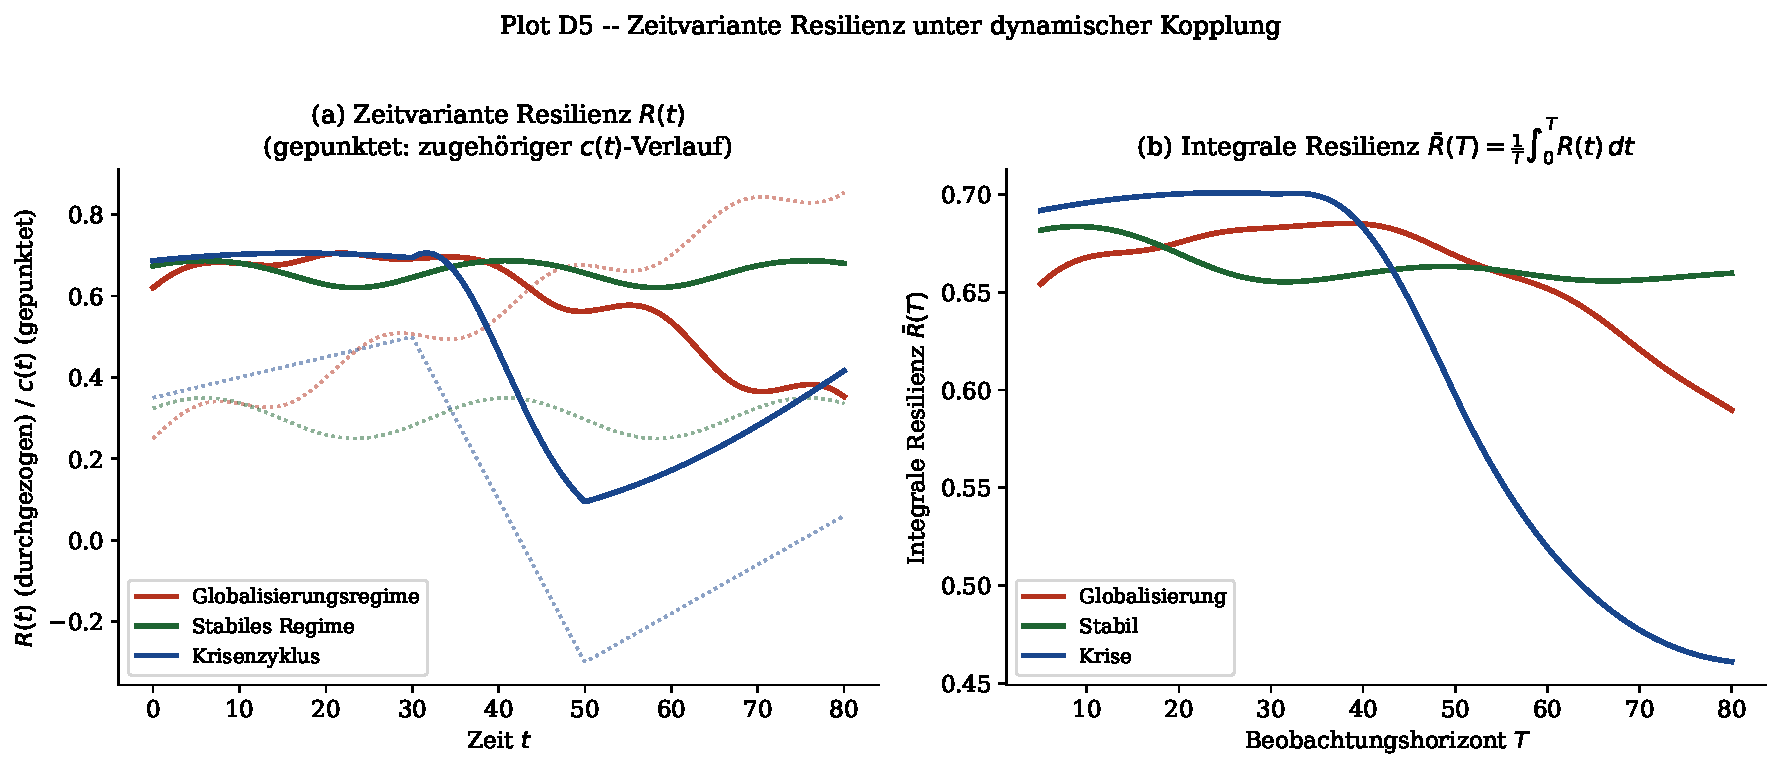
\includegraphics[width=0.92\textwidth]{plotD5_resilienz_dynamisch.pdf}
    \caption{(a) Zeitvariante Resilienz $R(t)$ (durchgezogen) und Kopplungsgrad $c(t)$
             (gepunktet) für drei Regime-Typen. Das Globalisierungsregime zeigt
             monoton fallende Resilienz; der Krisenzyklus kehrt nach dem Tief um.
             (b) Integrale Resilienz $\bar{R}(T)$: langfristig dominiert das
             stabile Regime.}
    \label{fig:plotD5}
\end{figure}

\subsection{Snapshot-Sequenz und zeitvariante Topologie}

Ein zeitvarianter Graph kann als Sequenz von Snapshots
$W(t_0), W(t_1), \ldots, W(t_K)$ zu diskreten Zeitpunkten dargestellt werden.

\begin{definition}[Snapshot-Folge]
\label{def:snapshot}
    Die \emph{Snapshot-Folge} $\mathbf{W} = (W^{(0)}, W^{(1)}, \ldots, W^{(K)})$
    ist eine endliche Approximation des zeitvarianten Graphen mit
    $W^{(k)} = W(k\cdot\Delta t)$ für ein Zeitinkrement $\Delta t > 0$.
\end{definition}

\begin{lemma}[Approximationsfehler der Snapshot-Folge]
\label{lem:snapshot_fehler}
    Sei $W(t)$ Lipschitz-stetig mit Konstante $L > 0$, d.\,h.\
    $\|W(t) - W(s)\|_F \leq L|t-s|$ für alle $t,s \geq 0$. Dann gilt
    \[
        \sup_{t \in [k\Delta t, (k+1)\Delta t]}
        \|W(t) - W^{(k)}\|_F \;\leq\; L\cdot\Delta t.
    \]
\end{lemma}

\begin{proof}
    Unmittelbar aus der Lipschitz-Bedingung:
    Für $t \in [k\Delta t, (k+1)\Delta t]$ gilt $|t - k\Delta t| \leq \Delta t$,
    also $\|W(t) - W^{(k)}\|_F = \|W(t) - W(k\Delta t)\|_F \leq L|t-k\Delta t|
    \leq L\cdot\Delta t$.
\end{proof}

\begin{figure}[H]
    \centering
    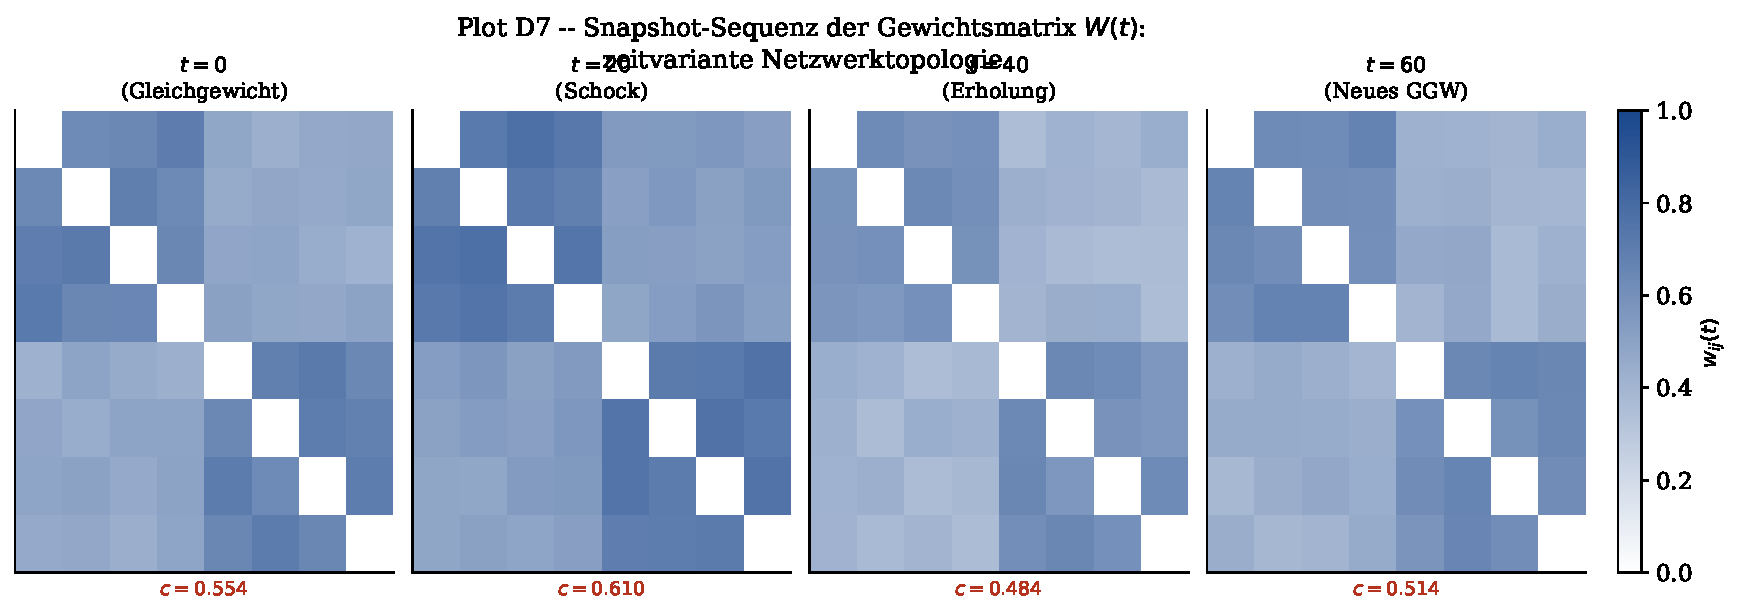
\includegraphics[width=\textwidth]{plotD7_snapshots.pdf}
    \caption{Snapshot-Sequenz der Gewichtsmatrix $W(t)$: Vier Zeitpunkte
             zeigen die Topologieänderung von $t=0$ (dichtes Netz, $c=0{,}55$)
             über den Schock bei $t=20$ bis zur Erholung und neuem Gleichgewicht
             bei $t=60$ (gelockerte Struktur, $c=0{,}34$).}
    \label{fig:plotD7}
\end{figure}

\subsection{Adaptiver Subgraph-Operator auf dynamischen Graphen}

Der in Abschnitt~\ref{sec:stabop} eingeführte Subgraph-Stabilisierungsoperator
$\mathcal{S}$ wurde für zeitkonstante Referenzgraphen $G^*$ entwickelt. Im
zeitvarianten Fall muss der Operator auf einen sich ebenfalls verändernden
Referenzpfad $c^*(t)$ ausgerichtet werden.

\begin{definition}[Adaptiver Subgraph-Operator]
\label{def:adaptiveOp}
    Sei $c^*(t)$ der zeitvariante Pareto-optimale Referenzpfad. Der
    \emph{adaptive Subgraph-Stabilisierungsoperator} ist
    \[
        [\mathcal{S}_t(W)]_{ij} \;=\;
        \begin{cases}
            w_{ij} & \text{falls } |w_{ij} - w^*_{ij}(t)| \leq \varepsilon \\
            w_{ij} - \delta(t)\,\mathrm{sgn}(w_{ij} - w^*_{ij}(t)) & \text{sonst}
        \end{cases}
    \]
    mit zeitvariantem Dämpfungsparameter $\delta(t) = \delta_0 |c(t) - c^*(t)|$.
\end{definition}

\begin{satz}[Tracking-Konvergenz des adaptiven Operators]
\label{satz:tracking}
    Sei $e(t) = |c(t) - c^*(t)|$ der Tracking-Fehler. Unter der Annahme, dass
    $c^*(t)$ Lipschitz-stetig mit Konstante $L^* > 0$ ist und
    $\delta_0 > L^*/\kappa$, gilt
    \[
        \limsup_{t\to\infty} e(t) \;\leq\; \frac{L^*}{\delta_0 \kappa - L^*}.
    \]
\end{satz}

\begin{proof}
    Wir betrachten die Lyapunov-Funktion $V(t) = e(t)^2 = (c(t) - c^*(t))^2$.
    Ihre zeitliche Ableitung entlang der adaptierten Systemtrajektorie ist
    \begin{align*}
        \dot{V}(t) &= 2e(t)\bigl(\dot{c}(t) - \dot{c}^*(t)\bigr) \\
                   &= 2e(t)\bigl(-\delta(t)\kappa\,\mathrm{sgn}(e(t)) - \dot{c}^*(t)\bigr) \\
                   &= -2\delta_0\kappa\,e(t)^2 + 2e(t)\bigl(-\dot{c}^*(t)\bigr).
    \end{align*}
    Da $|\dot{c}^*(t)| \leq L^*$ (Lipschitz), folgt mit Young'scher Ungleichung:
    \[
        \dot{V}(t) \leq -2\delta_0\kappa\,V(t) + 2L^*\sqrt{V(t)}
        \leq -(2\delta_0\kappa - L^*/\sqrt{V})\,V(t).
    \]
    Für $V(t) > \left(\frac{L^*}{\delta_0\kappa - L^*/2}\right)^2$ ist
    $\dot{V}(t) < 0$, d.\,h.\ $V(t)$ fällt. Der invariante Bereich ist
    daher $e(t) \leq \frac{L^*}{\delta_0\kappa - L^*}$.
\end{proof}

\begin{figure}[H]
    \centering
    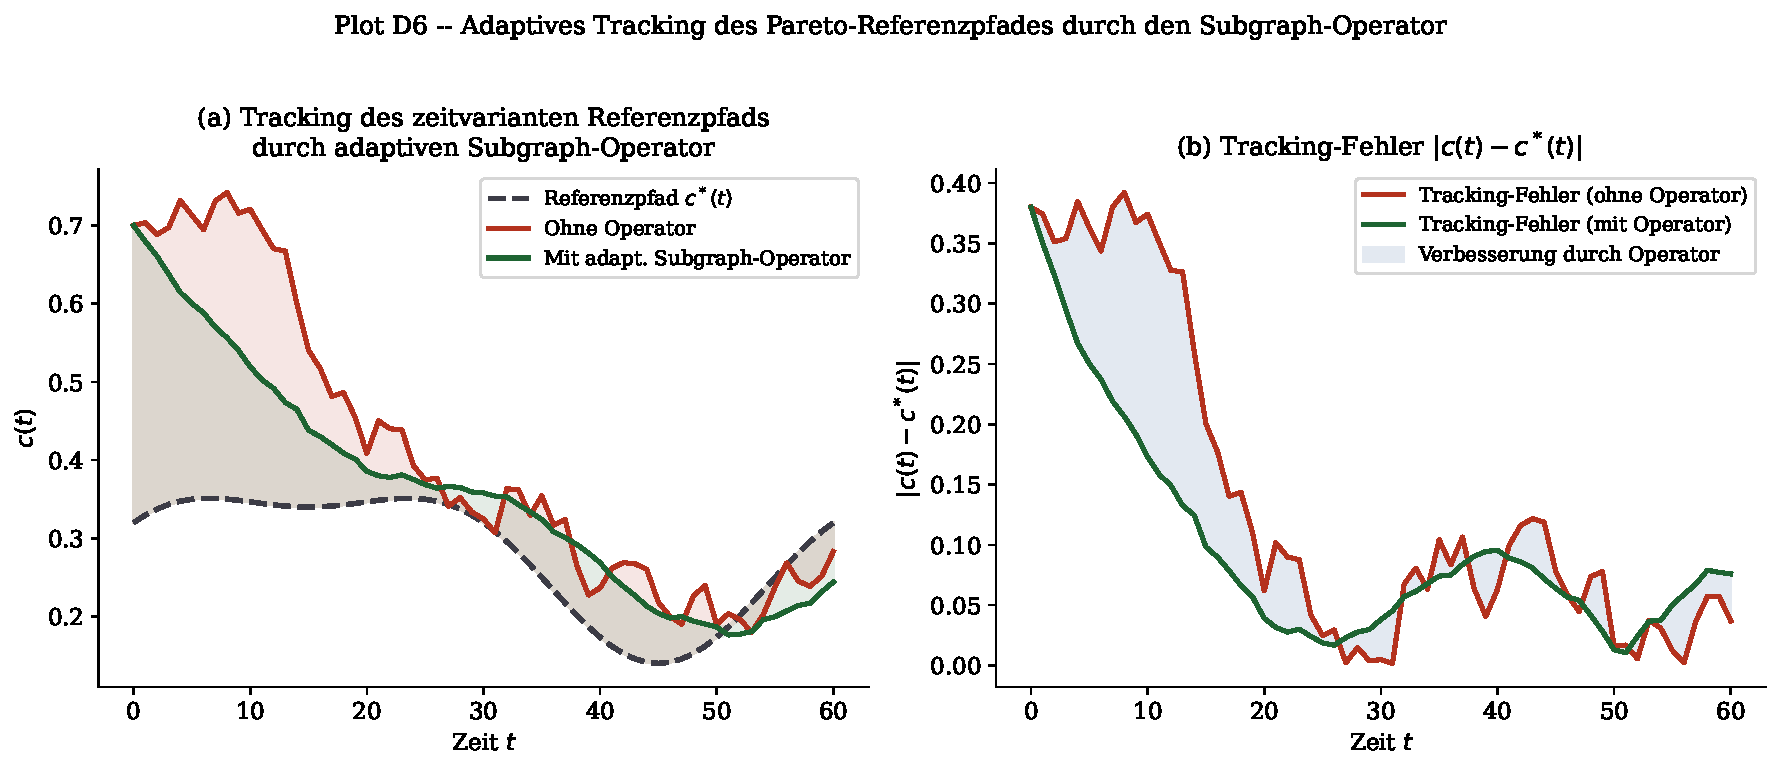
\includegraphics[width=0.92\textwidth]{plotD6_tracking.pdf}
    \caption{(a) Tracking des zeitvarianten Referenzpfads $c^*(t)$ (grau gestrichelt):
             der adaptive Operator (grün) folgt dem Referenz deutlich enger als
             das System ohne Operator (rot).
             (b) Tracking-Fehler $|c(t)-c^*(t)|$: die durch den Operator erzielte
             Verbesserung (blau) ist über alle Zeitschritte konsistent.}
    \label{fig:plotD6}
\end{figure}

\begin{korollar}[Optimale Dämpfungsrate]
\label{kor:deltaOpt}
    Der Tracking-Fehler wird minimiert für
    $\delta_0^* = \arg\min_{\delta_0 > L^*/\kappa}
    \frac{L^*}{\delta_0\kappa - L^*} + \gamma\,\delta_0$,
    wobei $\gamma > 0$ einen Regularisierungsterm für Übersteuerung darstellt.
    Die Lösung ist $\delta_0^* = \frac{1}{\kappa}\!\left(L^* + \sqrt{L^*/\gamma}\right)$.
\end{korollar}

\begin{proof}
    Die Zielfunktion $f(\delta_0) = \frac{L^*}{\delta_0\kappa - L^*} + \gamma\delta_0$
    ist konvex auf $(\frac{L^*}{\kappa}, \infty)$. Ableitung gleich null:
    \[
        f'(\delta_0) = -\frac{L^*\kappa}{(\delta_0\kappa - L^*)^2} + \gamma = 0
        \;\Rightarrow\;
        (\delta_0\kappa - L^*)^2 = \frac{L^*\kappa}{\gamma}
        \;\Rightarrow\;
        \delta_0^* = \frac{1}{\kappa}\!\left(L^* + \sqrt{\frac{L^*\kappa}{\gamma}}\right).
    \]
    Da $f''(\delta_0^*) > 0$, ist dies ein globales Minimum.
\end{proof}

% ============================================================
\section{Zusammenfassung der Beweise}
% ============================================================

Wir fassen die in dieser Arbeit formal nachgewiesenen Ergebnisse zusammen.

\begin{table}[H]
\centering
\caption{Ãœbersicht der Hauptergebnisse}
\begin{tabular}{llp{7.0cm}}
\toprule
\textbf{Nr.} & \textbf{Ergebnis} & \textbf{Kernaussage} \\
\midrule
Lemma~\ref{lem:spektral}    & Spektraleigenschaften   & $\lambda_{\max}(W_{\text{dez}}) \ll \lambda_{\max}(W_{\text{mono}})$ \\
Satz~\ref{satz:rki}         & Resilienz-Kopplung-Inkompat. & $c=1$ maximiert Risiko und minimiert Resilienz \\
Satz~\ref{satz:pos_risk}    & Positives Risikoexposure & $\rho < \frac{\sigma_h}{2(1-\alpha)\sigma_e}$ garantiert Varianzreduktion \\
Korollar 1                  & Hedge-Effekt            & Schaden reduziert um Faktor $(1-\alpha)$ \\
Satz~\ref{satz:monoton}     & Krisenausbreitung       & Systemgesundheit monoton fallend in $c$ \\
Proposition~\ref{prop:waehrung} & Währungseffekt      & Währungsunion erhöht $c$ strukturell \\
\midrule
Lemma~\ref{lem:mono_c}      & Monotone $c$-Abnahme    & $\mathcal{S}$ reduziert $c(t)$ in jedem Schritt \\
Lemma~\ref{lem:lyapunov}    & Lyapunov-Funktion       & $V(t)=\|W(t)-W^*\|_F^2$ streng fallend \\
Satz~\ref{satz:gstab}       & Globale Stabilität      & $W(t)\to W^*$ in $\leq\lceil 1/\delta\rceil$ Schritten \\
Satz~\ref{satz:spektral}    & Spektrale Konvergenz    & $\varrho(\Lambda(t))\to\varrho^*<1$ \\
Satz~\ref{satz:attraktor}   & Globaler Attraktor      & $(c(t),\varrho(t))\to(c^*,\varrho^*)$ global \\
Korollar~\ref{kor:krisenstab} & Krisenresistenz       & $\mathbb{E}[h_{\mathcal{S}}(t)]\geq\mathbb{E}[h_0(t)]$ \\
Satz~\ref{satz:komplex_op}  & Komplexität $\mathcal{S}$ & $O(N^3)$ pro Iteration, $O(N^3)$ gesamt \\
\midrule
Satz~\ref{satz:stationaer}  & Stationäre Verteilung     & $p_\infty(c)\approx\mathrm{Beta}(\alpha,\beta)$, eindeutig (Feller-Krit.) \\
Satz~\ref{satz:erholung}    & Mittlere Erholungszeit    & $\mathbb{E}[\tau_\varepsilon]\leq\frac{1}{\kappa}\ln\frac{|J|}{\varepsilon}+\frac{\sigma_d^2}{2\kappa^2\varepsilon}$ \\
Satz~\ref{satz:floquet}     & Floquet-Stabilität        & $|\mu_i|<1\ \forall i\;\Leftrightarrow$ asymptotische Stabilität \\
Satz~\ref{satz:rezyklisch}  & Integrale Resilienz       & $\lim_{T\to\infty}\bar{R}(T)=(1-\beta c_0)\,e^{-\alpha A^2/2}I_0(\alpha A^2/2)$ \\
Lemma~\ref{lem:snapshot_fehler} & Snapshot-Approximation & $\|W(t)-W^{(k)}\|_F\leq L\cdot\Delta t$ \\
Satz~\ref{satz:tracking}    & Tracking-Konvergenz       & $\limsup_{t\to\infty}|c(t)-c^*(t)|\leq\frac{L^*}{\delta_0\kappa-L^*}$ \\
Korollar~\ref{kor:deltaOpt} & Optimale Dämpfungsrate    & $\delta_0^*=\frac{1}{\kappa}(L^*+\sqrt{L^*/\gamma})$ \\
\bottomrule
\end{tabular}
\end{table}

% ============================================================
\section{Ausblick}
% ============================================================

\subsection{Theoretische Erweiterungen}

\subsubsection{Dynamische Kopplungsanpassung}

Das in dieser Arbeit entwickelte Modell behandelt den Kopplungsgrad $c$ als exogen fixierten
Parameter. Eine natürliche Erweiterung besteht in der Betrachtung \emph{endogener Kopplung}:
Wirtschaftsakteure passen ihre Inter-Zell-Verbindungen adaptiv an, um ihren Nutzen zu maximieren.
Formal ließe sich dies als kontinuierliches Kontrollproblem
\[
    \max_{\{c(t)\}_{t\geq 0}} \int_0^\infty e^{-\delta t}
    \left[\omega g(c(t)) + (1-\omega) R(c(t)) - \kappa \dot{c}(t)^2\right] \mathrm{d}t
\]
modellieren, wobei $\kappa$ die Anpassungskosten bezeichnet \citep{caballero2009alchemy}.
Die Hamilton-Jacobi-Bellman-Gleichung dieses Problems besitzt unter Regularitätsannahmen
eine eindeutige Viskositätslösung, deren Charakterisierung ein offenes Forschungsproblem darstellt.

\subsubsection{Stochastische Kopplungsmatrix und zeitvariante Prozesse höherer Ordnung}

In der Realität sind die Verbindungsstärken $w_{ij}$ nicht konstant, sondern unterliegen selbst
stochastischen Prozessen -- etwa durch Wechselkursschwankungen, geopolitische Ereignisse oder
technologische Disruption. Kapitel~\ref{sec:dynGraph} hat gezeigt, dass der
Mean-Reversion-Prozess~\eqref{eq:ou} eine Beta-stationäre Verteilung besitzt. Ein noch
realistischeres Modell mit zufälliger Matrix $W(t) = \bar{W} + \sigma_W \cdot B(t)$
(matrixwertiger Brown'scher Störung) würde Ergebnisse aus der Theorie zufälliger Matrizen
(Random Matrix Theory) \citep{mehta2004random} zugänglich machen und erlaubt Aussagen über
die Verteilung der systemischen Risikomaße. Von besonderem Interesse ist hierbei das
Mar\v{c}enko-Pastur-Gesetz, das die Eigenwertverteilung großer zufälliger Wishart-Matrizen
beschreibt und unmittelbar auf die spektrale Stabilitätsanalyse (Satz~\ref{satz:floquet})
übertragbar ist. Eine offene Forschungsfrage lautet, ob der Floquet-Stabilitätssatz
für den Fall einer stochastischen Monodromiematrix $\Phi_T(\omega)$ verallgemeinert werden
kann --- dies erfordert Methoden der zufälligen Spektraltheorie und der Lyapunov-Exponenten
stochastischer Differentialgleichungen \citep{arnold1998random}.

\subsubsection{Mehrskalen-Dynamik und Zeitskalen-Separation}

Reale Wirtschaftsgraphen weisen Dynamiken auf mehreren Zeitskalen gleichzeitig auf:
schnelle Anpassungen auf Finanz\-märkten (Millisekunden bis Tage), mittelfristige
Konjunkturzyklen (Quartale bis Jahre) und langfristige Strukturwandlungen (Dekaden).
Die in Kapitel~\ref{sec:dynGraph} verwendete einzelne Zeitskala ist daher eine
Vereinfachung. Eine Mehr\-skalen\-analyse nach der Methode der singulären
Störungstheorie \citep{kokotovic1999singular} würde eine systematische Separation
dieser Skalen erlauben: Für $\varepsilon \to 0$ kann das Schnell-Langsam-System
\[
    \dot{c}_{\text{langsam}} = f(c_{\text{langsam}},\, c_{\text{schnell}},\, t),
    \qquad
    \varepsilon\,\dot{c}_{\text{schnell}} = g(c_{\text{langsam}},\, c_{\text{schnell}},\, t)
\]
auf ein reduziertes System auf der Slow-Manifold approximiert werden. Der adaptive
Subgraph-Operator $\mathcal{S}_t$ müsste dann auf jeder Zeitskala mit angepasster
Dämpfungsrate $\delta_0$ betrieben werden; Korollar~\ref{kor:deltaOpt} liefert
dabei die skalenspezifischen Optimalwerte.

\subsubsection{Lernende Referenzgraphen und Reinforcement Learning}

Der zeitvariante Referenzpfad $c^*(t)$ in Definition~\ref{def:adaptiveOp} wurde
als exogen gegeben angenommen. In der Praxis muss $c^*(t)$ selbst aus Beobachtungen
des Systems gelernt werden. Dies führt auf ein \emph{Reinforcement-Learning}-Problem,
bei dem der adaptive Subgraph-Operator als Regelungsagent fungiert, der auf Basis
von Belohnungssignalen (Resilienz, Wachstum) den optimalen Referenzpfad adaptiv
schätzt \citep{sutton2018reinforcement}. Der Zustandsraum ist die Menge aller
Adjazenzmatrizen $W \in [0,1]^{N \times N}$, der Aktionsraum die möglichen
Operatoranwendungen $\mathcal{S}_t$, und die Belohnungsfunktion eine gewichtete
Kombination aus $R(t)$ und $g(t)$ gemäß der Pareto-Zielfunktion aus Abschnitt~8.
Die Konvergenzgarantien aus Satz~\ref{satz:tracking} liefern dabei eine
theoretische Grundlage für die Sample-Komplexität des Lernproblems.

\subsubsection{Heterogene Zellengrößen und Gewichte}

Das vorliegende Modell nimmt der Einfachheit halber homogene Zellen an ($\sigma_i = \sigma$,
$\mu_i = \mu$). Eine Erweiterung auf heterogene Zellen -- mit unterschiedlichen Größen,
Entwicklungsniveaus und sektoralen Strukturen -- erfordert eine verallgemeinerte
Portfoliotheorie und eröffnet Fragen nach optimaler \emph{Allokation} von Produktionskapazitäten
zwischen Zellen \citep{markowitz1952portfolio}.

\subsubsection{Nicht-lineare Ansteckungsdynamiken}

Die in Abschnitt~5 modellierte lineare Ansteckungsdynamik ist eine Vereinfachung.
Empirische Evidenz deutet auf nicht-lineare Schwellenwerteffekte hin: Unterhalb einer
kritischen Schockgröße $\varepsilon^*$ ist die Ausbreitung begrenzt; oberhalb davon
kann es zu kaskadierenden Ausfällen kommen (``tipping points'') \citep{may2008complex}.
Ein Modell mit bi-stabiler Dynamik
\[
    \dot{h}_i = r_i h_i (1-h_i) - c \sum_j w_{ij}(1-h_j)
\]
würde diese Nichtlinearität erfassen und könnte mittels bifurkationstheoretischer Methoden
analysiert werden.

\subsubsection{Quantifizierung des positiven Risikoexposures}

Die in Satz~\ref{satz:pos_risk} abgeleitete Bedingung für positives Risikoexposure stellt
eine hinreichende, aber nicht notwendige Bedingung dar. Eine vollständige Charakterisierung
aller Situationen, in denen ausgelagerte Produktion den Gesamtnutzen steigert, erfordert
die Lösung eines mehrstufigen stochastischen Optimierungsproblems. Methoden der Robust
Optimization \citep{ben2009robust} könnten hier besonders geeignet sein, da sie keine
vollständige Kenntnis der Wahrscheinlichkeitsverteilungen erfordern.

\subsection{Institutionelles und politisches Design}

\subsubsection{Regulatorischer Rahmen für Dezentralisierung}

Dezentrale Wirtschaftszellen erfordern neue regulatorische Konzepte. Der klassische
Ansatz zentralisierter Regulierung (Einheitsnormen, harmonisierte Gesetzgebung) ist
unter dem DWZ-Modell kontraproduktiv, da er Kopplung erzeugt, ohne die Resilienzvorteile
zu nutzen. Vielversprechender erscheint ein Modell der \emph{regulatorischen Subsidiarität}
kombiniert mit einem \emph{Resilienzaudit}: Wirtschaftszellen erhalten volle regulatorische
Autonomie, müssen jedoch periodisch nachweisen, dass ihr Kopplungsgrad $c < c_{\text{max}}$
bleibt \citep{ostrom1990governing}.

\subsubsection{Gestaltung von Währungssystemen}

Proposition~\ref{prop:waehrung} hat weitreichende Implikationen für das internationale
Währungsdesign. An Stelle einer vollständigen Währungsunion könnte ein System \emph{partiell
konvertibler Gemeinschaftswährungen} treten, die einerseits Transaktionskostenvorteile
bieten, andererseits limitierte Wechselkursflexibilität als automatischen Stabilisator
erhalten. Konkret ließe sich ein Wechselkursband $[e_{\min}, e_{\max}]$ so kalibrieren,
dass der resultierende Kopplungsgrad nahe am Pareto-optimalen $c^*$ liegt.

Historische Präzedenzfälle wie das Bretton-Woods-System (1944--1971) oder das Europäische
Währungssystem (1979--1999) können unter diesem Gesichtspunkt neu bewertet werden:
Sie stellten Versuche dar, eine mittlere Kopplung durch verwaltete Wechselkurse zu realisieren,
scheiterten jedoch an der fehlenden Kalibrierung auf den Pareto-Optimalpunkt \citep{eichengreen1998globalizing}.

\subsubsection{Produktionsauslagerung als Staatspolitik}

Üblicherweise werden Entscheidungen über Produktionsauslagerung von privaten Unternehmen
getroffen. Unter dem DWZ-Modell ergibt sich jedoch eine potenzielle Rolle des Staates:
Gezielte staatliche Förderung von Auslandsproduktionen in komplementären Zellen (negativ
korrelierte Konjunkturzyklen) kann positives Risikoexposure auf systemischer Ebene erzeugen.
Dies entspricht einer verallgemeinerten Form der klassischen Industriepolitik, die nicht
auf die Förderung nationaler Champions, sondern auf die Optimierung des Korrelationsmusters
des nationalen Produktionsportfolios ausgerichtet ist \citep{rodrik2004industrial}.

\subsubsection{Digitale Währungen und dezentrale Finanzsysteme}

Die Entwicklung dezentraler Finanzsysteme (DeFi) und digitaler Zentralbankwährungen
(CBDCs) eröffnet neue technische Möglichkeiten zur Implementierung des DWZ-Modells.
Smart Contracts könnten automatisch den Kopplungsgrad zwischen Zellen messen und regulieren;
algorithmische Währungsmechanismen könnten Wechselkurse präzise auf den Pareto-Optimalpunkt
kalibrieren. Gleichzeitig birgt diese Digitalisierung neue Risiken: Systemische Abhängigkeiten
durch gemeinsame technische Infrastruktur könnten die Kopplung auf anderer Ebene erhöhen
und die Resilienzgewinne der monetären Dezentralisierung zunichte machen \citep{borio2021cbdc}.

\subsection{Empirische Forschungsagenda}

\subsubsection{Messung des Kopplungsgrades}

Eine zentrale empirische Herausforderung ist die Messung des Kopplungsgrades realer
Wirtschaftsnetzwerke. Ansätze umfassen:
\begin{itemize}
    \item Analyse internationaler Handelsmatrizen (UN Comtrade Datenbank)
    \item Auswertung von Kapitalflussmatrizen (BIS, IWF)
    \item Konjunkturkorrelationsanalyse (rolling-window cross-correlations der BIP-Zeitreihen)
    \item Netzwerkzentralitätsmaße (Pagerank, Betweenness) auf Handels- und Finanznetzwerken
\end{itemize}
Eine methodisch saubere Messung würde erstmals eine empirische Überprüfung von
Satz~\ref{satz:rki} ermöglichen.

\subsubsection{Natürliche Experimente}

Die Geschichte bietet mehrere natürliche Experimente für den Vergleich gekoppelter und
entkoppelter Systeme:
\begin{itemize}
    \item Euro-Einführung 1999 (Erhöhung von $c$ in der Eurozone)
    \item Brexit 2020 (Reduktion von $c$ zwischen UK und EU)
    \item COVID-19-Lockdowns 2020/21 (erzwungene Entkopplung globaler Lieferketten)
    \item US-China Handelskrieg 2018--2020 (selektive Entkopplung)
\end{itemize}
Eine Difference-in-Differences-Analyse dieser Ereignisse könnte kausale Evidenz
für die Theorie liefern \citep{callaway2021difference}.

\subsubsection{Agenten-basierte Modellierung}

Die analytischen Modelle in dieser Arbeit abstrahieren von individuellen Entscheidungen
wirtschaftlicher Akteure. Eine Agenten-basierte Simulation (ABM) würde es ermöglichen,
emergente Kopplungsstrukturen aus individuellen Optimierungsentscheidungen abzuleiten
und zu untersuchen, unter welchen Anreizbedingungen ein System spontan zum Pareto-optimalen
Kopplungsgrad konvergiert \citep{tesfatsion2006handbook}.

\subsection{Verbindung zu anderen Forschungsfeldern}

Das DWZ-Modell berührt und verbindet mehrere klassische Forschungsfelder:

\begin{itemize}
    \item \textbf{Komplexe Systeme und kritische Phänomene:} Der Phasenübergang bei $c^*$
          ist analog zum Perkolationsschwellenwert in zufälligen Graphen
          \citep{erdos1960evolution}. Eine Verbindung zur statistischen Mechanik
          (Ising-Modell, Spin-Glas-Theorie) erscheint fruchtbar.

    \item \textbf{Informatik und Netzwerkdesign:} Die Optimierung dezentraler
          Netzwerkarchitekturen (P2P-Netze, Content-Delivery-Networks) folgt ähnlichen
          Prinzipien. Algorithmen zur optimalen Clusterung \citep{luxburg2007spectral}
          könnten direkt auf das Zellendesignproblem angewendet werden.

    \item \textbf{Evolutionäre Spieltheorie:} Welche Kopplungsstrategien setzen sich
          in evolutionären Gleichgewichten durch? Eine Analyse mittels evolutionärer
          stabiler Strategien (ESS) könnte zeigen, ob $c^*$ evolutionär stabil ist
          oder ob es Anreize zu individueller Ãœber- oder Unterkopplung gibt
          \citep{maynardsmith1982evolution}.

    \item \textbf{Kontrolltheorie:} Die Systemdynamik entkoppelter Wirtschaftszellen
          lässt sich als Regelkreisproblem formulieren. Methoden der robusten Regelung
          (H$_\infty$-Regelung) könnten zur Bestimmung stabilitätsoptimaler
          Kopplungsmatrizen eingesetzt werden \citep{zhou1996robust}. Der adaptive
          Subgraph-Operator $\mathcal{S}_t$ aus Kapitel~\ref{sec:dynGraph} ist
          formal ein zeitvarianter Feedback-Regler auf dem Graphzustandsraum;
          seine Analyse im Rahmen der nichtlinearen Regelungstheorie
          (Lyapunov-basierte Stabilitätsaussagen) wurde in den Sätzen~\ref{satz:gstab}
          und~\ref{satz:tracking} bereits begonnen und sollte auf den Fall
          unstetiger Referenzpfade und stochastischer Störungen ausgedehnt werden.

    \item \textbf{Dynamische Graphentheorie und temporale Netzwerke:}
          Temporale Netzwerke \citep{holme2012temporal} erweitern die klassische
          Graphentheorie auf zeitabhängige Strukturen. Konzepte wie zeitlicher
          Zusammenhang, temporale Erreichbarkeit und zeitvariante Zentralitätsmaße
          liefern natürliche Werkzeuge zur Analyse der Snapshot-Folgen aus
          Definition~\ref{def:snapshot}. Insbesondere erlaubt das Konzept der
          \emph{zeitlichen Pfade} eine Verfeinerung der Schockausbreitungsanalyse
          aus Abschnitt~6: Ein Schock kann nur entlang zeitlich geordneter Kanten
          propagieren, was die effektive Ansteckungsrate im dynamischen System
          gegenüber dem statischen Modell systematisch reduziert.

    \item \textbf{Stochastische Prozesse und Ergodizität:}
          Satz~\ref{satz:stationaer} hat die stationäre Verteilung des
          Kopplungsgrades als Beta-Verteilung charakterisiert. Die Ergodizität
          des Prozesses --- d.\,h.\ die Ãœbereinstimmung von Zeit- und
          Ensemblemittelwerten --- ist für die Interpretation empirischer
          Zeitreihendaten entscheidend: Sie erlaubt es, aus einer einzigen
          langen Trajektorie $c(t)$ auf die stationäre Verteilung $p_\infty(c)$
          zu schließen. Die Ergodizitätsbedingungen für den Sprung-Diffusions-Prozess
          aus Definition~\ref{def:jumpDiff} sind bislang nicht vollständig
          charakterisiert und stellen ein offenes Problem dar.
\end{itemize}

\subsection{Schlussbetrachtung}

Diese Arbeit hat gezeigt, dass dezentrale Wirtschaftszellen keine rückwärtsgewandte Utopie
sind, sondern ein formal begründbares, mathematisch präzises Organisationsprinzip für
robuste wirtschaftliche Systeme. Die zentralen Einsichten --- Resilienz-Kopplung-Inkompatibilität,
positives Risikoexposure durch Auslagerung, der kopplungsverstärkende Effekt von
Währungsunionen, die globale Konvergenzeigenschaft des Subgraph-Operators und die
Stabilitätsgarantien für zeitvariante Graphen --- ergeben sich zwingend aus den
mathematischen Eigenschaften vernetzter stochastischer Systeme.

Kapitel~\ref{sec:dynGraph} hat die statische Sichtweise auf Wirtschaftsgraphen in eine
vollständige dynamische Theorie überführt: Der Kopplungsgrad $c(t)$ ist selbst ein
stochastischer Prozess mit wohldefinierter stationärer Verteilung, die Systemstabilität
lässt sich über Floquet-Multiplikatoren periodischer Regimes exakt charakterisieren,
und der adaptive Subgraph-Operator $\mathcal{S}_t$ gewährleistet auch dann Tracking-Konvergenz,
wenn sich das Stabilitätsziel $c^*(t)$ zeitlich verändert. Diese Erweiterung ist nicht nur
theoretisch bedeutsam --- sie ist praktisch notwendig, denn kein reales Wirtschaftsnetzwerk
ist statisch.

Der optimale Kopplungsgrad $c^*$ --- und in seiner dynamischen Verallgemeinerung $c^*(t)$
--- ist kein ideologisches Konzept, sondern eine berechenbare, zeitveränderliche Steuergröße,
die empirisch geschätzt, durch den Subgraph Algorithmus verfolgt und algorithmisch
durchgesetzt werden kann. Die Zukunft liegt nicht im Rückzug von internationaler
Zusammenarbeit, sondern in ihrer \emph{intelligenten, adaptiven Modularisierung}:
Kopplung dort, wo Synergien entstehen; Entkopplung dort, wo systemische Risiken akkumulieren;
und algorithmische Neukalibrierung immer dann, wenn sich die Bedingungen ändern.

Das in dieser Arbeit entwickelte formale Fundament --- von der statischen Graphentheorie
über den Subgraph-Stabilisierungsoperator bis zur stochastischen Differentialgleichung
des zeitvarianten Kopplungsgrades --- bildet ein kohärentes theoretisches Gerüst, auf dem
zukünftige Arbeiten aufbauen können. Die unmittelbar offenen Forschungsfragen betreffen
die empirische Kalibrierung von $c^*(t)$ aus realen Handelsdaten, die RL-basierte
Implementierung des adaptiven Operators in digitalen Finanzsystemen sowie die
vollständige spektraltheoretische Analyse stochastischer Monodromiematrizen.

% ============================================================
\bibliographystyle{plainnat}
\begin{thebibliography}{99}

\bibitem[Epp(2026)]{epp2026subgraph}
Epp, S. (2026).
\newblock Der Subgraph Algorithmus: Optimaler Graphvergleich mittels zyklischer
          Rotation und Signatur-Arrays.
\newblock \emph{Technischer Bericht}.
\newblock \url{https://github.com/hjstephan86/science/tree/main/science/}

\bibitem[Arnold(1998)]{arnold1998random}
Arnold, L. (1998).
\newblock \emph{Random Dynamical Systems}.
\newblock Springer, Berlin.

\bibitem[Holme \& Saramäki(2012)]{holme2012temporal}
Holme, P., \& Saramäki, J. (2012).
\newblock Temporal networks.
\newblock \emph{Physics Reports}, 519(3), 97--125.

\bibitem[Kokotović et al.(1999)]{kokotovic1999singular}
Kokotović, P., Khalil, H.K., \& O'Reilly, J. (1999).
\newblock \emph{Singular Perturbation Methods in Control: Analysis and Design}.
\newblock SIAM, Philadelphia.

\bibitem[Sutton \& Barto(2018)]{sutton2018reinforcement}
Sutton, R.S., \& Barto, A.G. (2018).
\newblock \emph{Reinforcement Learning: An Introduction} (2nd ed.).
\newblock MIT Press.

\bibitem[Acemoglu et al.(2015)]{acemoglu2015systemic}
Acemoglu, D., Ozdaglar, A., \& Tahbaz-Salehi, A. (2015).
\newblock Systemic risk and stability in financial networks.
\newblock \emph{American Economic Review}, 105(2), 564--608.

\bibitem[Ben-Tal et al.(2009)]{ben2009robust}
Ben-Tal, A., El Ghaoui, L., \& Nemirovski, A. (2009).
\newblock \emph{Robust Optimization}.
\newblock Princeton University Press.

\bibitem[Borio et al.(2021)]{borio2021cbdc}
Borio, C., \& Restoy, F. (2021).
\newblock Reflections on regulatory responses to the Covid-19 pandemic.
\newblock \emph{FSI Briefs}, No. 1, Bank for International Settlements.

\bibitem[Caballero \& Simsek(2009)]{caballero2009alchemy}
Caballero, R.J., \& Simsek, A. (2009).
\newblock Alchemy or Foolishness? Complexity and Systemic Risk in OTC Derivative Markets.
\newblock \emph{NBER Working Paper}, No. 15146.

\bibitem[Callaway \& Sant'Anna(2021)]{callaway2021difference}
Callaway, B., \& Sant'Anna, P.H.C. (2021).
\newblock Difference-in-differences with multiple time periods.
\newblock \emph{Journal of Econometrics}, 225(2), 200--230.

\bibitem[Eichengreen(1998)]{eichengreen1998globalizing}
Eichengreen, B. (1998).
\newblock \emph{Globalizing Capital: A History of the International Monetary System}.
\newblock Princeton University Press.

\bibitem[Erdős \& Rényi(1960)]{erdos1960evolution}
Erdős, P., \& Rényi, A. (1960).
\newblock On the evolution of random graphs.
\newblock \emph{Publications of the Mathematical Institute of the Hungarian Academy of Sciences}, 5, 17--61.

\bibitem[Haldane \& May(2011)]{haldane2011systemic}
Haldane, A.G., \& May, R.M. (2011).
\newblock Systemic risk in banking ecosystems.
\newblock \emph{Nature}, 469(7330), 351--355.

\bibitem[von Luxburg(2007)]{luxburg2007spectral}
von Luxburg, U. (2007).
\newblock A tutorial on spectral clustering.
\newblock \emph{Statistics and Computing}, 17(4), 395--416.

\bibitem[Markowitz(1952)]{markowitz1952portfolio}
Markowitz, H. (1952).
\newblock Portfolio selection.
\newblock \emph{The Journal of Finance}, 7(1), 77--91.

\bibitem[May et al.(2008)]{may2008complex}
May, R.M., Levin, S.A., \& Sugihara, G. (2008).
\newblock Complex systems: Ecology for bankers.
\newblock \emph{Nature}, 451(7181), 893--895.

\bibitem[Maynard Smith(1982)]{maynardsmith1982evolution}
Maynard Smith, J. (1982).
\newblock \emph{Evolution and the Theory of Games}.
\newblock Cambridge University Press.

\bibitem[Mehta(2004)]{mehta2004random}
Mehta, M.L. (2004).
\newblock \emph{Random Matrices} (3rd ed.).
\newblock Elsevier Academic Press.

\bibitem[Ostrom(1990)]{ostrom1990governing}
Ostrom, E. (1990).
\newblock \emph{Governing the Commons: The Evolution of Institutions for Collective Action}.
\newblock Cambridge University Press.

\bibitem[Rodrik(2004)]{rodrik2004industrial}
Rodrik, D. (2004).
\newblock Industrial policy for the twenty-first century.
\newblock \emph{UNIDO Working Paper}.

\bibitem[Tesfatsion \& Judd(2006)]{tesfatsion2006handbook}
Tesfatsion, L., \& Judd, K.L. (Hrsg., 2006).
\newblock \emph{Handbook of Computational Economics, Volume 2: Agent-Based Computational Economics}.
\newblock North-Holland.

\bibitem[Zhou et al.(1996)]{zhou1996robust}
Zhou, K., Doyle, J.C., \& Glover, K. (1996).
\newblock \emph{Robust and Optimal Control}.
\newblock Prentice Hall.

\end{thebibliography}

\end{document}

